\documentclass[12pt]{article}

\usepackage[
	colorlinks=true,
	urlcolor=blue,
	linkcolor=black]
{hyperref}

%\usepackage{wasysym}
\usepackage[english]{babel}
\usepackage{tikz}
\pagestyle{empty}
%\usepackage[margin=0in,paperwidth=596pt,paperheight=842pt]{geometry}
\usepackage[all]{hypcap}

\usepackage{graphicx}
\graphicspath{ {./Images/} }

\usepackage{geometry}
\usepackage{xcolor}
\usepackage{amsmath}
\usepackage[some]{background}
\usepackage{lipsum}

\usepackage{graphicx} % Zum Einfügen von Grafiken
\usepackage{caption}  % Für anpassbare Bildunterschriften
\usepackage{subcaption} % Für Unterabbildungen, wenn nötig

\usepackage{amsfonts}
\usepackage{floatflt}
\usepackage{amssymb}
\usepackage{pgfplots}

\begin{document}

\begin{titlepage}
   \begin{center}
   \LARGE  
   \vspace{1.0cm}
       
   \textbf{Mathematische Grundlagen des Maschinellen Lernens (ML)}

   \vspace{1.0cm}
  
   \large       
   ---- Ausarbeitung zu einer Vorlesung ("Buch") ---
       
   
   \vspace{1.0cm}
   
   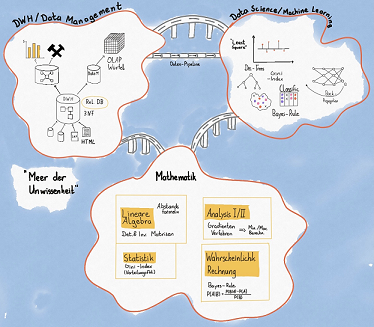
\includegraphics{DWH-Zeichnung}\\
   \small "3-Insel-Bild"  
   %\includegraphics{dhbw_logo} 
   %\begin{figure}
   %\epsfig{file=DHBW-Logo-BW.pdf, scale=0.1}
   %\end{figure}
       
   \vfill
   \large   
   
   Dr. Hermann Völlinger, Mathematik und IT Architektur
           \\ Stuttgart, Herbst 2023     

   \vspace{0.6cm}
        
   \end{center}
   
\begin{center}
Diese Version V0.6 (Datum: 30.8.2023) ist nicht final!!! \\
{\color{red}{(Beachte: ************ Kommentare *********)}} \\[0.3cm]
Aktuelle Versionen findet man in meinem GitHub\\[0.1cm]
\url{https://github.com/HVoellinger/Mathematische-Grundlagen_von_ML/blob/main/Math+MaschLernen(ML)v0.6.pdf} \\
\vspace{0.4cm}
\begin{large}
Dieses Skript wurde generiert mit \LaTeX\  
\end{large}
\end{center}

%\includegraphics[width=0.4\textwidth]{dhbw.gif}
% Department Name\\ Fakultät Technik-Informatik
  
\end{titlepage}

\begin{LARGE} Inhaltsangabe \end{LARGE}

\setcounter{tocdepth}{2}
\tableofcontents

\newpage
 
%\renewcommand{\labelenumi}{(\alph{enumi})}
%\renewcommand{\labelenumii}{\arabic{enumii}.}


\section{Management Zusammenfassung}

Ziel der Ausarbeitung ist es, die {\color{blue}mathematischen Konzepte des Maschinellen Lernens (ML)} zu erkennen.\\
Leider wird in der gängigen Literatur dieses Thema nicht genug gewürdigt. Dies mag damit zu tun haben das heutzutage mathematische Ausbildung in der Schule und in der Universität etwas den Bezug zur Realität verloren hat und deshalb viele Schüler und Studenten den Nutzen und die Schönheit der Mathematik nicht erkennen können. Es gehört ja manchmal schon "zum guten Ton", wenn technische Hochschulabsolventen fast schon scherzhaft sagen, dass Sie mit Mathematik "nichts am Hut haben". Dies ist leider sehr schade und ist zudem beim Lösen von ML Fragestellungen ein große Hürde.\\ Ein Ziel der Ausarbeitung ist es deshalb zu zeigen wie nützlich mathematische Ideen bei der Lösung der Fragestellungen des Maschinellen Lernens (aka: \url{https://en.wikipedia.org/wiki/Machine_learning}) sind.Die mathematischen Grundlagen des Machine Learning umfassen mehrere Bereiche der Mathematik, die für das Verständnis und die Entwicklung von Machine Learning Algorithmen von Bedeutung sind.
Hier sind einige wichtige \textbf{mathematische Konzepte und Grundlagen:}\\
\\
\textbf{1. Lineare Algebra:} Lineare Algebra ist ein grundlegender Bestandteil von Machine Learning. Vektoren und Matrizen werden verwendet, um Daten darzustellen, und Operationen wie Skalierung, Addition, Multiplikation und Transformationen werden angewendet, um Berechnungen durchzuführen. Matrixoperationen wie Matrixmultiplikation und Matrixinversion sind wichtig für viele Algorithmen.\\[0.2cm]
%
\textbf{2. Differentialrechnung:} Differentialrechnung wird verwendet, um Funktionen zu analysieren und Optimierungsalgorithmen abzuleiten. Berechnung von Gradienten, Ableitungen, partielle Ableitungen und Optimierungsmethoden wie das Verfahren zum Gradientenabstieg sind entscheidend für das Trainieren von Modellen und das Anpassen von Parametern.\\[0.2cm]
%
\textbf{3. Wahrscheinlichkeitstheorie und Statistik:} Wahrscheinlichkeitstheorie und Statistik spielen eine wichtige Rolle im Machine Learning, insbesondere im Bereich des überwachten und nicht überwachten Lernens. Wahrscheinlichkeitsverteilungen, Schätzungen, Hypothesenbildung und statistische Modelle werden verwendet, um Muster in den Daten zu erkennen, Vorhersagen zu treffen und Unsicherheiten zu quantifizieren.\\[0.2cm]
%
\textbf{4. Optimierung:} Optimierungsmethoden werden verwendet, um Modelle zu trainieren und die besten Parameterwerte zu finden. Die Optimierungstechniken umfassen lineare Programmierung, konvexe Optimierung und nichtlineare Optimierung.\\[0.2cm]
%
\textbf{5. Informationstheorie:} Informationstheorie befasst sich mit der Quantifizierung und Übertragung von Informationen. Konzepte wie Entropie, Informationsgewinn und Kompressionsalgorithmen spielen eine Rolle in der Modellierung und Auswahl von Merkmalen sowie in der Reduzierung der Komplexität von Daten.\\[0.2cm]
%
Diese mathematischen Grundlagen werden verwendet, um Modelle zu definieren, Daten zu analysieren, Funktionen anzupassen, Vorhersagen zu treffen und Modelle zu evaluieren. Sie dienen als Grundlage für das Verständnis der Algorithmen und Methoden des Machine Learning. Es ist wichtig, ein solides Verständnis dieser mathematischen Konzepte zu haben, um Machine Learning effektiv anzuwenden und weiterzuentwickeln.\\
%
\\ *** Weitere Kapitel Texte *** \\[0.2cm]
%
Mathematik ist eine Säule des maschinellen Lernens. Vor etwa 250 Jahren begann man, sie zu formalisieren, aber erst vor etwa 100 Jahren wurde die moderne Mathematik entwickelt. Es handelt sich um ein riesiges Fachgebiet, mit vielen Unterbereichen, wie Lineare Algebra, Statistik, etc. sowie mit Anwendungen in den Ingenieurwissenschaften und der Physik.\\
Zum Glück müssen wir nicht die ganze Breite und Tiefe der Mathematik kennen, um unser Verständnis und unsere Anwendung des maschinellen Lernens zu verbessern. Die wesentlichen Bereiche der Mathematik die näher betrachten werden, sind:\\

1.	Lineare Algebra für Maschinelles Lernen (ML)\\ 

2.	Wahrscheinlichkeitsrechnung und Statistische Methoden für ML\\ 

3.	Optimierungsmethoden für ML\\

4.	Analysis (i.e. "Gradienten-Verfahren") für ML\\[0.5cm]
%
Die wichtigsten ML Anwendungen und Methoden, die mathematische Verfahren nutzen, werden vorgestellt und in ihren wesentlichen Merkmalen erläutert.\\
Es werden zahlreiche Hinweise auf vertiefende Anwendungen oder Informationen durch Internet-Links oder weiterführende Literatur gegeben. An vielen Stellen werden konkrete Umsetzungsbeispiele mit Werkzeugen wie \textit{KNIME Analytics Platform} gezeigt. \\
Die Beziehungen ("Brücken") zwischen Mathematik, Maschinellen Lernen (ML) und Data Science (DL) (insbesondere \href{https://en.wikipedia.org/wiki/Data_mining}{Data Mining} werden konkret gebaut und anschließend beispielhaft "beschritten" (siehe auch "3-Insel-Bild" von der Titelseite).\\ 
Die Leser sollen befähigt werden, die Mathematik hinter den ML Anwendungen zu verstehen um mögliche weitere sinnvolle Ergänzungen und Erweiterungen die sich aus dem mathematischen Erkenntnisse ergeben zu nutzen.\\
Zu jedem Kapitel gibt es Übungen, die das im Kapitel Gelernte nochmals an konkreten Fragestellungen und Problemen erproben und vertiefen. Musterlösungen bzw. Hinweise zur Lösung der Übungen findet man am Ende des Buches.\\
Insgesamt beinhaltet die Arbeit zur Zeit 11 Kapitel.\\
\\
*** Weitere Kapitel Texte *** 


\newpage

\section{Wichtige Anwendungen der Mathematik in ML}

In diesem Skript/Buch werden Sie unter anderen sechs konkrete Beispiele für Mathematik bei bekannten Verfahren des Maschinellen Lernen (ML) kennenlernen. Pro Verfahren gibt es ein separates Kapitel im Skript\\
Die einzelne Kapitel werden durch anschauliche Beispiele motiviert und  ergänzt. Anhand dieser Beispiele kann mal auch schnell und anschaulich die allgemeinen mathematischen Grundlage der entsprechenden ML Verfahren nachvollziehen.\\
Zu den einzelnen Kapitel Themen gibt es jeweils mehrere Übungen bzw. Hinweise zu deren Lösung.\\
Diese sechs ML Verfahren sind:\\

%\begin{enumerate}
%\item[\color{blue}{1. text}]
%\item \blue{\item[2. text]
%\item[3. text]
%\end{enumerate}

1. Mathematik zum k-Means-Algorithmus ("Euklidische Distanz")\\

2. Entscheidungsbäume und GINI Index (Statistik)\\

3. Lineare Regression und "Best Fit" Verfahren der Analysis (AN)\\

4. Text-Klassifikation mit Bayes-Verfahren (Bedingte Wahrscheinlichkeiten)\\
 
5. Verfahren der "Support Vector Machines" (SVM)\\

6. Neuronale Netzwerke und Backpropagation via "Absteigende Gradienten"\\[0.2cm]
%
Am Ende kommt noch ein Kapitel \textbf{Anhang} in den sechs weitere ML-Verfahren der Vollständigkeit halber eher kurz erläutert werden. Diese sind:\\

1. Empfehlungssysteme "Recommender Systems" (LinAlgebra)\\

2. Regularisierungen "Regularization" und Lin. Algebra (LA)\\

3. Hauptkomponenten-Analyse "Principal Component Analysis" (PCA)\\
 
4. Singulärwertzerlegung "Singular Value Decomposition" (SVD)\\
 
5. Mathematische Verfahren im NLP, i.e. "Latent Semantic Analysis/Indexing (LSI)"?\\

6. Mathematik und grosse Sprachmodelle "Large Language Models" (LLMs))

\newpage

\section{Mathematik zum "k-Means-Algorithmus"}

Ein \textbf{k-Means-Algorithmus}ist ein Verfahren der Euklidischen Geometrie. Dabei wird aus einer Menge von ähnlichen Objekten eine vorher bekannte Anzahl von k Gruppen ("Clustern") gebildet.\\
Der Algorithmus ist eine der am häufigsten verwendeten Techniken zur Gruppierung von Objekten, da er schnell die Zentren der Cluster findet. Dabei bevorzugt der Algorithmus Gruppen mit geringer Varianz und ähnlicher Größe.\\
Der Algorithmus hat starke Ähnlichkeiten mit dem "Erwartungs-Maximierungs-Algorithmus (EM-Algorithmus)" und zeichnet sich durch seine Einfachheit aus.\\
Erweiterungen sind der $"k-Median-Algorithmus"$ und der $"k-Means++ Algorithmus" $.\\

\subsection{Problemstellung und Mathematik}

Ziel von k-Means ist es einen den Datensatz so in $k$ Partitionen zu teilen, dass die Summe der quadrierten Abweichungen von den Cluster-Schwerpunkten minimal ist. Mathematisch entspricht dies der Optimierung der Funktion:\\[0.2cm]
$ J = \sum_{i=1}^{k}  \sum_{\mathbf x_j \in S_{i}} {\| \mathbf x_j - \boldsymbol \mu_i \|^2}$ mit den Datenpunkten $ \mathbf x_j $ und den "Schwerpunkten" $ \boldsymbol \mu_i $ der Cluster $ S_i$.\\[0.2cm]
Diese Zielfunktion basiert auf der \textbf{Methode der kleinsten Quadrate} und man spricht auch von "Clustering durch Varianzminimierung", da die Summe der Varianzen der Cluster minimiert wird.\\
Da zudem $ \| \mathbf x_j - \boldsymbol \mu_i \|^2 $ die quadrierte "Euklidische Distanz" ist, ordnet k-Means effektiv jedes Objekt dem nächstgelegenen (nach Euklidischer Distanz) Clusterschwerpunkt zu.\\ 

\newpage
%
\begin{figure}[htp]
  \centering
  \hspace*{-0.1cm} 
  \includegraphics[width=0.7\textwidth]{k-Means-Konvergenz-Iteration0}
  \caption{k-Means-Konvergenz-Iteration0}
  \label{fig:k-Means-Iteration0}
\end{figure}
%
Um eine Animation einer 3-Means-Konvergenz mit 15 Iterationen zu sehen können sie auch folgenden Link aufrufen:\\
\url{https://github.com/HVoellinger/Mathematische-Grundlagen_von_ML/blob/main/Images/k-Means-Konvergenz-Animation.gif}\\

\subsection{k-Means Algorithmen}

Da die Suche nach der optimalen Lösung schwer ist, wird im Normalfall ein approximativer Algorithmus verwendet wie die \textbf{ Heuristiken von Lloyd oder MacQueen}. Da die Problemstellung von k abhängig ist, muss dieser Parameter vom Benutzer festgelegt werden\\

\subsubsection{Lloyd-Algorithmus}

Der am häufigsten verwendete k-Means-Algorithmus ist der \textbf{Lloyd-Algorithmus}, der oft als "der k-Means-Algorithmus" bezeichnet wird, obwohl Lloyd diesen Namen nicht verwendet hat. Lloyds Algorithmus besteht aus drei Schritten:\\[0.2cm]
\textbf{1. Initialisierung:} Wähle $k$ zufällige Mittelwerte ("Means"): $ \mathbf m_1^{(1)}, \ldots, \mathbf m_k^{(1)} $ aus dem Datensatz.\\
\textbf{2. Zuordnung:} Jedes Datenobjekt wird demjenigen Cluster zugeordnet, bei dem die Cluster-Varianz am wenigsten erhöht wird.
\begin{center}
$ S_i^{(t)} = \left\{ \mathbf x_j : \big\| \mathbf x_j - \mathbf m^{(t)}_i \big\|^2 \leq \big\| \mathbf x_j - \mathbf m^{(t)}_{i^*} \big\|^2 \text{ für alle }i^*=1,\ldots,k \right\}$\\[0.2cm]
\end{center}
\textbf{3. Aktualisieren:} Berechne die Mittelpunkte der Cluster neu.
\begin{center}
$ \mathbf m_i^{(t+1)} = \frac{1}{|S_i^{(t)}|} \sum_{\mathbf x_j \in S_{i}^{(t)}} \mathbf x_j  $ \\
\end{center}
Die Schritte 2–3 werden dabei so lange wiederholt, bis sich die Zuordnungen nicht mehr ändern.

\subsubsection{MacQueen'sLloyd-Algorithmus} 

MacQueen führte mit dem Begriff k-Means einen anderen Algorithmus ein:
\\[0.3cm]1. Wähle die ersten $k$ Elemente als Clusterzentren.\\
2. Weise jedes neue Element dem Cluster zu, bei dem sich die Varianz am wenigsten erhöht, und aktualisiere das Clusterzentrum.
\\[0.3cm]Während es ursprünglich – vermutlich – nicht vorgesehen war, kann man auch diesen Algorithmus iterieren, um ein besseres Ergebnis zu erhalten.

\subsection{Python Programm zum k-Means-Clustering}

{\color{red}{***********************************************************************\\ 
Ab hier bis Ende der Section sind die Folien der Vorlesung ML  zu nutzen und diese sind in Latex umzusetzen...\\
************************************************************************}}\\[0.2cm]


\begin{center}
\hspace*{-2.0cm}   
\includegraphics[width=1.0\textwidth]{K-Means-Python-Bild1}
\hspace*{-2.0cm}   
\includegraphics[width=1.0\textwidth]{K-Means-Python-Bild2}
\hspace*{-2.0cm} 
\includegraphics[width=1.0\textwidth]{K-Means-Python-Bild3}
\hspace*{-2.0cm} 
\includegraphics[width=1.0\textwidth]{K-Means-Python-Bild4}
\end{center}

\subsection{k-Means-Clustering für IRIS Blumen}


Der in diesem Beispiel verwendete Datensatz ist der berühmte IRIS-Datensatz. Er besteht aus 150 Einträgen der Irisblume, die jeweils durch vier Merkmale beschrieben werden: Kelchblattlänge, Kelchblattbreite, Blütenblattlänge und
Blütenblattbreite. \\
Zusätzlich ist der spezifische Typ der Irisblume angegeben. Es gibt drei Arten
der Schwertlilienpflanze: Iris Setosa, Iris Versicolor und Iris Virginica. Jede Art ist mit mit 50 Einträgen im Datensatz vertreten. Die Merkmale sind in Zentimetern angegeben. Die Abbildung unten zeigt wie die Daten im Datenrahmen dargestellt werden. Der Datensatz wurde erstmals von Ronald Fisher, einem britischen Biologen, in einem Aufsatz aus dem Jahr 1936 vorgestellt. Er ist eines der am häufigsten verwendeten Beispiele für statistischen Klassifizierung-Algorithmen beim Maschinellen Lernen. \\
Die Abbildung unten zeigt die ersten fünf Einträge des Datensatzes. Der Datensatz ist in der Python-Bibliothek scikit-learn enthalten.\\ 

\begin{figure}[htp]
  \centering
  \hspace*{-0.1cm} 
  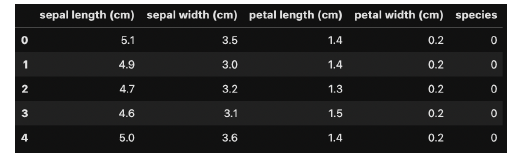
\includegraphics[width=0.7\textwidth]{IRIS-Dataset-First_Entries}\\
  \caption{Die ersten 5 Entries im IRIS Datensatz}
  \label{fig:Iris_DS}
\end{figure}
%...
Siehe Lösungen in meinem Github:\\ 
%
\url{https://github.com/HVoellinger/Mathematische-Grundlagen_von_ML/blob/main/Quellen_Math-ML/k-means-HVoe.pdf} \\
%
\url{https://github.com/HVoellinger/Mathematische-Grundlagen_von_ML/blob/main/Quellen_Math-ML/k-means-HVoe.tex}\\[0.3cm]
%
Die Konfusion-Matrix zeigt, dass alle 50 setosa-Blüten richtig klassifiziert  wurden. 48 versicolor-Blüten wurden richtig klassifiziert, aber 14 wurden falsch erkannt). 36 virginica-Blüten wurden richtig beschriftet und 2 virginica-Blüten wurden fälschlicherweise als virginica-Blüten klassifiziert.\\
%
Insgesamt funktionieren  Clustering und Klassifizierung mit k-Means im IRIS-Datensatz gut. Mit einer Genauigkeit von 89% ist der Algorithmus ein gutes Hilfsmittel, um ein Modell für die Vorhersage der genauen Art der Irisblüte zu erstellen.\\
Wie die Konfusion-Matrix zeigt, ist die Klassifikation zu 100% genau
für die Setosa-Blüten und über 94 % für die Versicolor-Arten. Es scheitert nur bei der genauen Virginica-Blüten mit einer Genauigkeit von "nur" 77 %.\\
Das Modell von k-Means kann jedoch noch weiter verbessert werden, wie andere  Implementierungen wie k-means++ zeigen. Es verbessert außerdem die Wahl der anfänglichen Zentren.

\newpage

{\color{red}{***********************************************************************\\ 
Ab hier bis Ende der Übungen sind die Folien der Vorlesung ML  zu nutzen und diese sind in Latex umzusetzen...\\
************************************************************************}}\\[0.2cm]
\subsection{Übungen zum Kapitel 3}
.....\\
\subsubsection{Übung 3.1 - nnn1}
TEXT\\
\subsubsection{Übung 3.2 - nnn2}
.....\\
\subsubsection{Übung 3.3 - ...............}


\newpage

\section{Lernen von Entscheidungsbäumen / "Decision Tree" (DT) Learning}


\textbf{Entscheidungsbaum-Algorithmen} sind weit verbreitete Methoden im maschinellen Lernen, die zur \textbf{Klassifikation und Regression} verwendet werden.\\

\subsection{Mathematik bei Entscheidungsbäumen}

Es gibt verschiedene mathematische Verfahren und Techniken, die bei der Konstruktion und Optimierung von Entscheidungsbäumen eingesetzt werden. Hier sind einige davon:\\
%
\textbf{1. Entropie und Informationsgewinn:}\\
Die Entropie ist ein Maß für die Unordnung oder Unsicherheit in einem Datensatz. Beim Konstruieren eines Entscheidungsbaums wird der Informationsgewinn verwendet, um festzustellen, wie gut eine Funktion (Attribut) den Datensatz in Bezug auf die Zielvariable aufteilt. Der Informationsgewinn wird oft in Form von Entropieänderungen zwischen den ursprünglichen und den aufgeteilten Datensätzen gemessen.
%
\textbf{2. Gini-Index:}\\
Der Gini-Index misst die Wahrscheinlichkeit, dass eine zufällig ausgewählte Instanz falsch klassifiziert wird, wenn sie zufällig nach den Klassenverteilungen in einem Teilbaum ausgewählt wird. Ein niedriger Gini-Index deutet auf eine homogene Verteilung der Klassen hin.\\
%
\textbf{3. Reduktion des quadratischen Fehlers (Regression):}\\
Bei Entscheidungsbäumen für Regression werden mathematische Kriterien wie die Reduktion des quadratischen Fehlers verwendet, um die besten Aufteilungen der Daten zu finden, die zu einer geringeren Varianz der Zielvariablen führen.\\
%
\textbf{3. Cost-Complexity-Pruning:}\\
Nach dem Konstruieren eines Entscheidungsbaums können zu viele Verzweigungen zu Overfitting führen. Das Cost-Complexity-Pruning verwendet eine Kostenfunktion, um die Qualität eines Baums in Bezug auf seine Komplexität zu bewerten. Durch Entfernen von Verzweigungen, die nur geringfügig zur Verbesserung der Modellgenauigkeit beitragen, kann die Generalisierungsfähigkeit des Baums verbessert werden.\\
%
\textbf{4. CART (Classification and Regression Trees):}\\
Der CART-Algorithmus verwendet eine rekursive Zweig- und Bindemethode, um einen Baum zu erstellen. Er sucht nach der besten Spaltung eines Datensatzes anhand des Gini-Index (für Klassifikation) oder der Reduzierung des quadratischen Fehlers (für Regression).\\
%
\textbf{5. Random Forests und Boosting:}\\
Diese Ansätze basieren auf Entscheidungsbäumen, werden jedoch durch die Kombination mehrerer Bäume oder das Hinzufügen von Gewichten zu den Instanzen verbessert. Sie nutzen mathematische Methoden, um die Vorhersagegenauigkeit und Robustheit zu erhöhen.\\
%
\textbf{5. Hyperparameter-Optimierung:}\\
Die Wahl der Hyperparameter, wie beispielsweise die maximale Tiefe des Baums oder die Mindestanzahl der Instanzen in einem Blatt, beeinflusst die Leistung des Entscheidungsbaums. Mathematische Verfahren wie Rastersuche oder Bayes'sche Optimierung können verwendet werden, um die besten Hyperparameter für das Modell zu finden.\\[0.2cm]
%
\textbf{Zusammenfassung}:
Diese Verfahren sind alle Teil des Prozesses der Konstruktion, Anpassung und Optimierung von Entscheidungsbäumen im maschinellen Lernen. Die Wahl des geeigneten Verfahrens hängt von der Art des Problems und den Daten ab, mit denen Sie arbeiten.\\

\subsection{Mathematische Grundlagen Gini-Index- und Entropie-Verfahren }


\subsubsection{Gini-Index Verfahren}

{\color{red}{*******************************************************************\\ 
ab hier bis Ende der section sind die Folien der Vorlesung ML  zu nutzen und diese sind in Latex umzusetzen\\
********************************************************************\\}}



\subsubsection{Entropie: ID3-Verfahren}


\textbf{Iterative Dichotomiser3 (ID3)} ist ein Algorithmus, der zur Entscheidungsfindung bei Entscheidungsbäumen eingesetzt wird.\\
Der australische Forscher [[J. Ross Quinlan]] publizierte diesen Algorithmus erstmals im Jahr 1986. ID3 war in seinen ersten Jahren sehr einflussreich. Er findet auch heute noch in einigen Produkten Verwendung. ID3 gilt als Vorgänger des [C4.5]-Algorithmus.\\
%
ID3 wird verwendet, wenn bei großer Datenmenge viele verschiedene Attribute von Bedeutung sind und deshalb ein Entscheidungsbaum ohne große Berechnungen generiert werden soll. Somit entstehen meist einfache Entscheidungsbäume. Es kann aber nicht garantiert werden, dass keine besseren Bäume möglich wären.\\[0.2cm]
%
\textbf{Mathematischer Algorithmus} \\[0.2cm]
Die Basisstruktur von ID3 ist iterativ. Es werden zu jedem noch nicht benutzten Attribut Entropien bezüglich der Trainingsmenge berechnet. Das Attribut mit dem höchsten Informationsgewinn (Englisch: \textit{Information Gain IG}) bzw. der kleinsten Entropie, wird gewählt und daraus ein neuer Baum-Knoten generiert.\\
Das Verfahren terminiert, wenn alle Trainingsinstanzen klassifiziert wurden, d.h. wenn jedem Blattknoten eine Klassifikation zugeordnet ist.\\[0.1cm]
Der Informationstheoretische Verständnis des Begriffes \textbf     {Entropie} geht auf [Claude Elwood Shannon] zurück und existiert seit etwa 1948. In diesem Jahr veröffentlichte Shannon seine fundamentale Arbeit "A Mathematical Theory of Communication"\\ (\url{http://math.harvard.edu/~ctm/home/text/others/shannon/entropy/entropy.pdf})
 und prägte damit die moderne Informationstheorie.\\
Die Entropie wird üblicherweise mit einem großen griechischen Eta  \text{H} bezeichnet. Claude Elwood Shannon definierte die Entropie $ \mathrm{H} $ einer diskreten, gedächtnislosen Quelle (diskreten Zufallsvariable) $ X $ über einem endlichen, aus Zeichen bestehenden Alphabet $ Z=\{z_1, z_2, \dots, z_m\}$ wie folgt: \\
Zunächst ordnet man jeder Wahrscheinlichkeit $ p $ eines Ereignisses seinen Informationsgehalt $ I(z) = -\log_2 p_z $ zu. Dann ist die \textbf{Entropie eines Zeichens} definiert als der Erwartungswert des Informationsgehalts: \
\begin{center}
$ \mathrm{H_1} = E[I]= \sum_{z\in Z} p_z I(z) = - \sum_{z\in Z} p_z \log_2 p_z $.\\
\end{center}
Sei $ z \in Z $, dann ist $ p_z = P(X=z) $ die Wahrscheinlichkeit, mit der das Zeichen $ z $ des Alphabets auftritt, oder gleichwertig:\\ 
\begin{center}
$ \qquad \mathrm{H_1} = - \sum_{i=1}^{m} p_i \log_2 p_i $ mit $ p_i = p_{z_i} $ 
\end{center}
Dabei wird $ 0\cdot\log_2 0=0 $ gesetzt (entsprechend dem Grenzwert $  \lim_{x \rightarrow 0} x \log_2 x $. Summanden mit verschwindender Wahrscheinlichkeit tragen daher aufgrund der Definition nicht zur Summe bei.\\
Die Entropie $ \mathrm{H_n} $ für Wörter $ w $ der Länge $ n $ ergibt sich durch:
\begin{center}
$ (1) \qquad \mathrm{H_n} = -\sum_{w \in Z^n} p_w \log_2 p_w $
\end{center}
wobei $ p_w  = P(X=w)$ die Wahrscheinlichkeit ist, mit der das Wort $  w $ auftritt. \\
Die Entropie $ \mathrm{H} $ ist dann der Grenzwert der Folge $ n\to \infty $ davon:
\begin{center}
$ (2)\qquad \mathrm{H} = \lim_{n\to \infty} \frac {\mathrm{H_n}}{n} $.
\end{center}
Wenn die einzelnen Zeichen stochastisch voneinander unabhängig sind, dann gilt $ \mathrm{H_n} = n \mathrm{H_1} $ für alle $ n $, also $ \mathrm{H} = \mathrm{H_1} $. Vergleiche auch Blockentropie:\\
\url{https://de.wikipedia.org/wiki/Bedingte_Entropie#Blockentropie}.\\[0.3cm]
% 
\textbf{Auswahl der Attribute ("Merkmale"):}\\[0.2cm]
Sei $ T $ die Menge der Trainingsbeispiele mit ihrer jeweiligen Klassifizierung, $ a \in A $ das zu prüfende Attribut aus der Menge der verfügbaren Attribute, $ V(a) $ die Menge der möglichen Attributwerte von $ a $ und $ T_ v$ die Untermenge von $ T $, für die das Attribut $ a $ den Wert $ v $ annimmt. Der Informationsgewinn, der durch Auswahl des Attributs $ a $ erzielt wird, errechnet sich dann als Differenz der Entropie von $ T $ und der erwarteten durchschnittlichen Entropie von $ T $ bei Fixierung von $ a $:\\[0.2cm]
\begin{center}
$ IG(T, a) = \operatorname{Entropie}(T) - \sum_{v \in V(a)} \dfrac{|T_v|}{|T|} \operatorname{Entropie} (T_v) $. \\
\end{center}
Schließlich wählt man ein Attribut mit dem größtmöglichen Gewinn aus der Menge 
\begin{center} 
$\lbrace a_{next} \in A | IG(T, a_{next}) = \max_{a \in A}(IG(T, a)) \rbrace $ 
\end{center}
als das nächste Attribut.\\[0.2cm]
Diese Wahl führt zur Bevorzugung von Attributen mit vielen Wahlmöglichkeiten und damit zu einem breiten Baum. Um dem entgegenzuwirken kann eine Normalisierung über die Anzahl der Wahlmöglichkeiten durchgeführt werden.\\
Siehe auch folgenden Weblink:\\
\url{https://github.com/HVoellinger/Mathematische-Grundlagen_von_ML/blob/main/Quellen_Math-ML/Homework_H4.5-DecTree_ID3_Praesentation.pdf}\\[0.2cm]


\subsection{Beispiele für Gini-Index- und Entropie-Verfahren }


\subsubsection{Beispiele für Gini-Index Verfahren}

{\color{red}{***********************************************************************\\ 
Ab hier bis Ende der Section sind die Folien der Vorlesung ML  zu nutzen und diese sind in Latex umzusetzen...\\
************************************************************************}}\\[0.2cm]



\hspace*{-1.8cm}
\includegraphics[width=595.4401pt,height=841.32pt]{latexImage_f093f131e1ba361d5f674df0ed2570f1.png}

\hspace*{-1.8cm}
\includegraphics[width=595.4401pt,height=841.32pt]{latexImage_763b10c1e5a667e05d9d13d585345751.png}

\subsubsection{Beispiel für Entropie-Verfahren}

\begin{center}
\hspace*{-3.0cm}   
\includegraphics[width=1.4\textwidth]{DT-Entropie-Bild1}
\hspace*{-2.5cm}   
\includegraphics[width=1.4\textwidth]{DT-Entropie-Bild2}
\hspace*{-2.5cm} 
\includegraphics[width=1.4\textwidth]{DT-Entropie-Bild3}
\hspace*{-2.5cm} 
\includegraphics[width=1.4\textwidth]{DT-Entropie-Bild4}
\end{center}


\url{https://github.com/HVoellinger/Mathematische-Grundlagen_von_ML/blob/main/Quellen_Math-ML/Homework_H4.5-DecTree_ID3.pdf}

\subsection{GINI-Index "Production Maintenance"}


{\color{red}{***********************************************************************\\ 
Ab hier bis Ende Subsection sind die Folien der Vorlesung ML  zu nutzen und diese sind in Latex umzusetzen...\\
************************************************************************}}\\[0.2cm]



\newpage


\subsection{Übungen zu Kapitel 4}
{\color{red}{***********************************************************************\\ 
Ab hier bis Ende der Übungen sind die Folien der Vorlesung ML  zu nutzen und diese sind in Latex umzusetzen...\\
************************************************************************}}\\[0.2cm]


\subsubsection{Übung 4.1}
\begin{figure}[htp]
  \centering
  \hspace*{-1.5cm} 
  \includegraphics[width=1.2\textwidth]{DT-Homework(1+2)}
  \caption{DT-Homework(1+2)}
\label{fig:DT_Learning1}
\end{figure}

\subsubsection{Übung 4.2}

\subsubsection{Übung 4.3}

\begin{figure}[htp]
  \centering
  \hspace*{-1.5cm} 
  \includegraphics[width=1.2\textwidth]{DT-Homework(3+4)}
  \caption{DT-Homework(3+4)}
\label{fig:DT_Learning2}
\end{figure}

\subsubsection{Übung 4.4}


\subsubsection{Übung 4
.5}

\begin{figure}[bp]
  \centering
  \hspace*{-1.5cm} 
  \includegraphics[width=1.2\textwidth]{DT-Homework5}
  \caption{DT-Homework5}
\label{fig:DT_Learning2}
\end{figure}


\newpage

\section{Lineare Regression (LR) in ML }

\subsection{Allgemeine Einführung in Regressionsmodelle}

Ein \textbf{Regressionsmodell im Machine Learning} ist ein statistisches Modell, das dazu verwendet wird, die Beziehung zwischen einer abhängigen (oder Ziel-) Variable ("Target") und einer oder mehreren unabhängigen (oder erklärenden) Variablen (Features") zu analysieren und zu beschreiben. Das Hauptziel der Regression besteht darin, Vorhersagen für die abhängige Variable zu treffen, basierend auf den Werten der unabhängigen Variablen.\\
Die Grundidee hinter einem Regression ist es, eine Funktion zu finden, die die bestmögliche Anpassung an die gegebenen Daten bietet. Je nach Art der Daten und der Beziehung zwischen den Variablen gibt es verschiedene Arten von Regressionsmodellen, darunter:\\[0.2cm] 
% 
1. \textbf{Lineare Regression}: Hierbei handelt es sich um das einfachste Regressionsmodell, bei dem versucht wird, eine lineare Beziehung zwischen den unabhängigen und abhängigen Variablen zu finden.\\[0.2cm]
%  
2. \textbf{Polynominale - oder auch Multidim. Regression}: Diese erweitert die lineare Regression, indem sie Polynome höheren Grades verwendet, um komplexere Beziehungen zwischen den Variablen zu modellieren.\\[0.2cm]
% 
3. \textbf{Logistische Regression}: Obwohl der Name "Regression" enthält, wird die logistische Regression hauptsächlich für Klassifikation Probleme verwendet, bei denen die abhängige Variable diskrete Werte annimmt. Sie wird verwendet, um die Wahrscheinlichkeit zu schätzen, dass eine bestimmte Klasse in einem binären oder mehrklassigen Klassifikationsproblem auftritt.\\[0.2cm]
%  
4. \textbf{Ridge Regression und Lasso Regression}: Diese Varianten der linearen Regression dienen dazu, mit möglicherweise hochdimensionalen Datensätzen umzugehen und Overfitting zu reduzieren, indem sie Regularisierungstechniken verwenden.\\[0.2cm] 
% 
5. \textbf{Nichtlineare Regression}: Für komplexere Zusammenhänge zwischen den Variablen werden nichtlineare Regressionsmodelle verwendet, die nichtlineare Funktionen verwenden, um die Daten besser anzupassen.\\[0.2cm]
% 
6. \textbf{Zeitreihenregression}: Diese Art der Regression wird verwendet, um Zeitreihendaten zu modellieren, bei denen die abhängige Variable über einen Zeitverlauf hinweg beobachtet wird.\\[0.2cm]
% 
\textbf{Zusammenfassung}: Die Auswahl des geeigneten Regressionsmodells hängt von der Natur der Daten, der Art der Beziehung zwischen den Variablen und den Zielen der Analyse ab.\\Die Modellierung und Auswertung von Regressionsmodellen sind grundlegende Techniken im Bereich des maschinellen Lernens und werden in einer Vielzahl von Anwendungen eingesetzt, von der Vorhersage von Aktienkursen bis zur medizinischen Diagnose.\\[0.2cm] 

{\color{red}{******* Beispiel von Latex Syntax für eine Tabelle und ein Matrix  *******}}\\[0.2cm]


\begin{table}[h] % Tabelle wird hier eingefügt, wenn möglich
  \centering
  \begin{tabular}{|c|c|}
    \hline
    Spalte 1 & Spalte 2 \\
    \hline
    Inhalt 1 & Inhalt 2 \\
    \hline
  \end{tabular}
  \caption{Eine Tabelle mit Positionsangabe "h".}
  \label{tab:tabelle_h}
\end{table}


Berechnen Sie die Determinante der Matrix:
\\[0.1cm]
\begin{center}
\hspace*{0.1cm}

$ A := \left(
   \begin{array}{llll}
     1 & 2 & 3 & 4 \\
     2 & 3 & 4 & 1 \\ 
     3 & 4 & 1 & 2 \\ 
     4 & 1 & 2 & 3 \\ 
   \end{array}
   \right) $ 
%\caption{Darstellung einer 4x4 Matrix}
%\label{tab:Matrix_4x4)}
\\[0.3cm]
\end{center} 
{\color{red}{******* Ende Beispiel von Latex Syntax für eine Tabelle und eine Matrix *******}}\\[0.2cm] 
 

\subsection{Motivation und Beispiele der Linearen Regression}

In unserem Skript fokussieren wir uns auf die \textbf{Lineare Regressionen (LR)}.
Das LR Modell geht von einer linearen Beziehung zwischen den Variablen aus, was bedeutet, dass Änderungen in den unabhängigen Variablen ("Features") mit konstanten Veränderungen in der abhängigen Variable (Target") einhergehen.\\
Die lineare Regression nutzt eine Methode, die als \textbf{"Methode der kleinsten Quadrate"} bezeichnet wird, um die besten Schätzwerte für die Koeffizienten zu finden. Diese Methode minimiert die quadratischen Abweichungen zwischen den beobachteten Werten und den vom Modell vorhergesagten Werten. \\
Sei k die Anzahl der unabhängigen Variablen dann sprechen wir bei k = 1 von einer {\color{blue}{"Einfachen (simple) Linearen Regression" (sLR)}} und bei $k\geqslant 2.$ von einer {\color{blue}{"Multidimensionalen (multiplen) Linearen Regression"(mLR)}}.\\
Eine Trainingsmenge von n Datenpunkten $\lbrace P_j \rbrace$ in $\mathbb{R}^{k+1} $ wird dargestellt als Vektor: 
\begin{center}
$ \lbrace(x_{ij},y_j) \rbrace$,  wobei $1 \leq i \leq k $ und $1 \leq j \leq n $.\\
\end{center} 
Die ersten k Komponenten $\lbrace x_{ij} \rbrace $ pro Datenvektor sind die Komponenten der unabhängigen Variablen ("Features") und die letzte Komponente $ \lbrace(y_j)\rbrace $ ist die Komponente der abhängigen Variable ("Target" oder auch "Label").\\  Mit anderen Worten (aus fachlicher Sicht) sollen aus den k Eigenschaften $\lbrace x_{ij} \rbrace$ eine Aussage über die Zieleigenschaft $\lbrace y_j \rbrace$ gemacht werden.   

\subsubsection{Beispiele von LR Lösungen für k=1, k=2}

Mathematisch ("Geometrie") erhalten wir für k=1 eine Gerade in $ \mathbb{R}^2 $. \\
%
Wir schreiben die \textbf{Geradengleichung} als $ y = a + b \cdot x $. \\
$a$ ist dabei der Achsenabschnitt ("y-intercept" auf Englisch) und $b$ die Steigung in x-Richtung ("x-slope").\\[0.2cm] 
%
Für k = 2 eine Ebene in $ \mathbb{R}^3$ mit der \textbf{Ebenengleichung} $ z  = a + b \cdot x  + c \cdot y $. \\
$a$ ist dabei der Achsenabschnitt mit der z-Achse (z-intercept), $b$ die Steigung in x-Richtung (x-slope) und $c$ die Steigung in y-Richtung (y-slope) \\[0.2cm] 
%
Für $k \eqslantgtr 3 $ erhalten wir eine Hyperebene in $ \mathbb{R}^{k+1}$.     \\[0.4cm]
%
Die ersten zwei Fälle lassen sich leicht visualisieren:\\[0.3cm] 
\textbf{k=1:} Das folgende Bild zeigt die $ \color{red}{"Regressionsgerade"} $ für die n blauen Beobachtungspunkte $ \color{blue}{\lbrace P_1 = (x_1,y_1)\quad...\quad P_n = (x_n,y_n) \rbrace } $
\\[0.2cm]
\hspace*{0.2cm}
\begin{center}
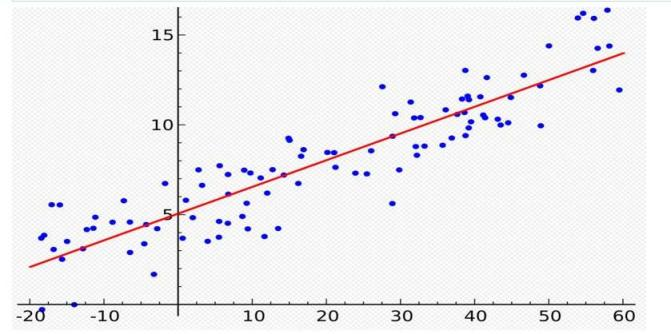
\includegraphics{sLR-Gerade} 
\end{center}
\textbf{k=2:} Das nächste Bild zeigt die $ \color{black}{"Regressionsebene"} $ für die n blauen Beobachtungspunkte $ \color{blue}{\lbrace P_1 = (x_1, y_1, z_1)\quad ... \quad P_n = (x_n, y_n, z_n)\rbrace } $
\begin{center}
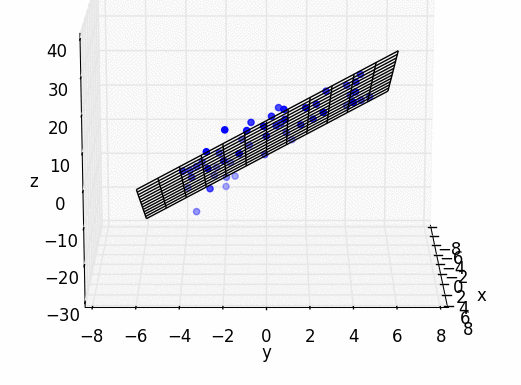
\includegraphics{ML5-MovingPicture_mLR}\
\end{center} 
Ein bewegtes Bild davon liegt in der Referenz [HVö-5]: 
\url{https://github.com/HVoellinger/Lecture-Notes-to-ML-WS2020/blob/master/ML5-QYuIc.gif}
.....\\


\subsection{Kennzahlen  $ R^2 $ und $ adj.{R^2} $ }

Für die Definition der \textbf{simple Linear Regression (sLR)} und \textbf{multiple Linear Regression (mLR)} brauchen wir einige Kennzahlen für die Datenpunkte (i.e."Beobachtungspunkte") aus der Trainingsmenge (\textit{observation points}).\\
Diese Kennzahlen sind \textbf{Sum of Squares Total (SST), Sum of Squares Error (SSE)} und \textbf{Sum of Squares Regression (SSR)}.\\ 

\subsubsection{Definition der sLR Kennzahl $ R^2 $}

Die Definition der Kennzahl $R^2$ benutzt die Kennzahlen SST und SSE). SSR wird für die eigentliche Definition von $R^2$ nicht genutzt. Wir brauchen diese Kennzahl aber später im Kapitel. Definiere der Einfachheit halber: 
\begin{center}
$ f_i = f(x_i)$ und $\overline{y} = \frac{1}{n} \sum\limits_{i=1}^n \Bigl(y_i \Bigr) $,   wobei n = (Anzahl der Beobachtungen)
\end{center} 
SST, SSE und SSR sind gegeben durch die folgenden Definitionen. Ohne Verlust der Allgemeinheit (o.A.) können wir dabei annehmen das SST größer als Null ist:
\begin{center}
$ \texttt{(D-4.1): Sum of Squares Total (SST) := } \sum\limits_{i=1}^n \Bigl(y_i - \overline{y})\Bigr)^2 $ 
$ \texttt{(D-4.2): Sum of Squares Error (SSE) := } \sum\limits_{i=1}^n \Bigl(y_i - f_i\Bigr)^2 $
$ \texttt{(D-4.3): Sum of Squares Regression (SSR) := } \sum\limits_{i=1}^n \Bigl(f_i - \overline{y})\Bigr)^2 $  
\end{center}
% Zeilenfüller
Für die Definition von R² brauchen wir Sum of Squares Error (SSE) und Sum of Squares Total (SST). Die Definition von R² ist gegeben durch die Differenz von 1 und dem Quotienten SSE/SST. Wir nennen R² in Deutsch auch "Bestimmtheitsgrad":\\
\begin{center}
\texttt{(D-4.4):}
\begin{Large}  
\textbf{$ R^2 := 1 - \frac{SSE}{SST} $} \\[0.8 cm]
\end{Large}   
\end{center}
% Zeilenfüller
\textbf{Sprechweise:} Wir sagen eine Gerade ist eine \textbf{"optimale"} (sLR)-Gerade wenn R² maximal ist (dies ist analog zu SSE ist minimal). Oftmals wird in der Literatur auch der Zusatz "optimale" weggelassen und man sagt nur "sLR-Gerade".\\[0.2 cm]
% Zeilenfüller
%\textbf{Anmerkung:} Wir sehen später das für  optimale sLR-Geraden eine andere Formel für R² auch gültig ist. Diese Formel benutzt die Kennzahl SSR.\\[0.4cm]
% Zeilenfüller
Im \textbf{folgenden Bild} sehen wir die Kennzahlen {\color{blue}{SSE}} und {\color{red}{SST}} geometrisch mit 4 Beobachtungspunkten. Sehr gut sind die Größen der Quadrate für {\color{blue}{SSE}} und {\color{red}{SST}} zu erkennen. Man bekommt zudem auch ein guten Eindruck von den Faktor 
\begin{large}
$ \frac{\color{blue}{SSE}}{\color{red}{SST}} $\\[5.8cm]
\end{large}

\begin{figure}[htp]
\hspace*{-1.0cm}  
\centering 
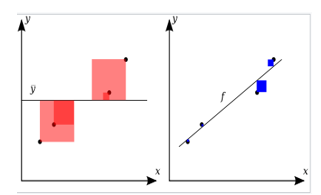
\includegraphics[width=0.8\textwidth]{SSE_SST-Definition}
  \caption{Geometrische Darstellung von {\color{blue}{SSE}} und {\color{red}{SST}}}
  \label{fig:SSE-SST-1}
\end{figure}


\subsubsection{Eigenschaften und Theoreme zu $R^2$ } 

Nun wollen wir die ersten offensichtlichen mathematische Aussagen zu R² machen. \\
Zur leichteren Schreibweise nutze ich die folgenden Notationen:\\
\begin{center}
sum(xi):= $ \sum\limits_{i=1}^n(x_i) $ und Mean(x) = $ \overline{x} := \frac{1}{n} \cdot \sum\limits_{i=1}^n(x_i) $\\[0.2cm]
\end{center}
Wir beginnen mit einigen einfachen mathematischen Aussagen ("Theoreme", "Propositionen", "Korollare", etc. ) über die Eigenschaften der Kennzahl $R^2$.\\[0.2cm]
\textbf{Anmerkung:} Ohne Einschränkung der Allgemeinheit ("OE") können wir annehmen, dass $SST > 0$ ist.\\[0.2cm] 
%
\textbf{Theorem (Th-4.1)}: "Eigenschaften von $R^2$”\\[0.2cm]
Es gelten die folgenden Aussagen:\\[0.3cm]
(i)  $ \quad 0 \leqslant R^2 \leqslant 1 \quad\quad\quad\quad\quad\quad $   "Begrenzung"\\[0.2cm]                                       
(ii) $ \quad R^2 = 0 \Leftrightarrow SSE = SST \quad $                      "Minimum"\\[0.2cm]                                       
(iii) $ \quad R^2 = 1 \Leftrightarrow SSE = 0 \quad\quad\quad $                 "Maximum"\\[0.4cm]                                       
\textbf{Beweis:}
Der Beweis dieser Aussagen ist trivial. Um aber das mathematische Kalkül einzuüben führen wir hier die mathematische Beweisargumentation explizit aus:\\[0.2cm]
ad (i): per Definition gilt $ SST \geqslant SSE \Leftrightarrow 1 \geqslant \frac{SSE}{SST} \Leftrightarrow 1- \frac{SSE}{SST} \geqslant 0 \Leftrightarrow R^2\geqslant 0 $\\[0.2cm]                                       
per Definition gilt $ \frac{SSE}{SST} \geqslant 0 \Leftrightarrow 0 \geqslant -\frac{SSE}{SST} \Leftrightarrow 1 \geqslant 1- \frac{SSE}{SST} \frac{SSE}{SST} R^2 \leqslant 1 $ \\[0.3cm]                                       
ad (ii): $ SSE = SST \Leftrightarrow \frac{SSE}{SST} = 1 \Leftrightarrow 1 - \frac{SSE}{SST} = 0 \Leftrightarrow R^2 = 0 $ \\[0.2cm]                                                                           
ad (iii): $SSE = 0 \Leftrightarrow \frac{SSE}{SST} = 0 \Leftrightarrow  1 + \frac{SSE}{SST} = 1 \Leftrightarrow  1 = 1 -  \frac{SSE}{SST} \Leftrightarrow  R^2 = 1 \qquad $ q.e.d. \\[0.3cm] 
%
Manchmal ist es notwendig das die optimale sLR-Gerade durch den Ursprung (a=0) geht. In diesem Fall erhalten wir die folgende Aussage:\\
\\[0.2cm]
\textbf{Korollar(K-4.1)}: “opt. sLR ohne Achsenabschnitt(a =0)”\\
\begin{center}
\begin{large}
Aus $ a=0 \Rightarrow b = {\dfrac{\overline{x \cdot y}}{\overline{x^2}}}$  \\[0.2cm]                                          
\end{large}
\end{center}
\textbf{Beweis:}\\
$ a = 0 \Rightarrow y = b \cdot x$\\\\[0.1cm]
%                                                                           
Da die sSLR-Gerade optimal ist, nuss die Ableitung von $R^2$ nach b gleich Null. Berechne nun diese. Da die Ableitung von SST konstant ist und die Gleichung später = 0 gesetzt wird, gilt: 
\begin{center}
\begin{large}
$ 0 =\frac{\partial}{\partial b} (1-\frac{SSE}{SST}) = \frac{\partial)}{\partial b} [SSE] = \frac{\partial}{\partial b}[\sum\limits_{i=1}^n [(y_i - b \cdot x_i)^2] = -2 \cdot \sum(y_i \cdot x_i - b \cdot (x_i)^2) $ 
\end{large}
\end{center}
daraus folgt:
\begin{center}
\begin{large}
$ \sum(y_i \cdot x_i) =  b \cdot \sum(x_i)^2) \Rightarrow b = \frac{\sum(y_i \cdot x_i) }{\sum(x_i)^2)} \Rightarrow m = \frac{\overline{x \cdot y}}{\overline{x^2}} \qquad $ q.e.d.     \\[0.5cm] 
\end{large}
\end{center} 
%
Wir brauchen für später auch noch weitere hilfreiche Formeln über Summen und Mittelwerte. Diese werden für die Berechnung der “optimalen” Koeffizienten $a$ und $b$ gebraucht (siehe: “Least Square Fit” (LSF) Methode):\\[0.8cm]
{\color{red}{***********************************************************************\\ 
Ab hier bis Ende der subsection sind die Folien der Vorlesung ML  zu nutzen und diese sind in Latex umzusetzen...\\
***************************************************************************}}
\\[0.2cm]                                                                                                                                      
%                                                                                                                                     
\textbf{Proposition (P-4.1)}:\\[0.2cm] 
Easily you can proof, that the following equations are valid \\
(definiere M(x):=Mean(xi))\\[0.2cm] 
(i)  Sum[(xi - M(x))²] = sum(xi²) - n*M(x)² \\[0.2cm]
(ii) Sum[(yi – M(y))²] = sum(yi²) - n*M(y)² \\[0.2cm]
(iii) Sum[(xi - M(x))*(yi - M(y))] = sum(xi*yi) – n*M(x)*M(y)\\[0.2cm]
\textbf{Beweis:}\\[0.2cm]
 ”straightforward”:\\[0.2cm]
%
(i) sum[(xi - M(x))²] = sum[xi²- 2*M(x)*(xi) + M(x)²]   (binominal formula) 
        = sum(xi²)- 2*M(x)* sum(xi)+ sum(M(x)²)= sum(xi²)– 2*n*M(x)²+ n*M(x)²    weil sum(xi)=n*M(x))\\[0.2cm]  
%         
(ii) analog: sum[(yi-M(y))]²= sum(yi²)-2*M(y)*sum(yi)+ sum[M(y)²]=sum(yi²) - 2n*M(y)²+n*M(y)² = sum(yi²)- n*M(y)\\[0.2cm]
%
(iii) analog: sum[(xi-M(x))*(yi-M(y))]= sum[xi*yi- M(x)*yi– xi*M(y)+ M(x)*M(y)]     (durch Ausmultiplizieren aller Faktoren)\\         
  = sum(xi*yi)– n*M(x)*M(y)- n*M(x)*M(y)+ n*M(x)*M(y) = sum(xi*yi*)-n*M(x)*M(y)\\q.e.d.\\
  

\subsubsection{Definition der mLR-Kennzahl adj.R²}

In diesem Abschnitt definieren wir die Theorie der \href{https://en.wikipedia.org/wiki/Linear_regression}{"mutiple linear regression"}.\\
In einem {\color{blue}{multiplen Regression Problem}} arbeiten wir mit $n$ Datenpaaren $\langle\mathbf{x}^{(i)}, y^{(i)} \rangle \in \mathbb{R}^{k+1} $ 
wobei $\mathbf{x}^{(i)} \in \mathbb{R}^k$ und $y^{(i)} \in \mathbb{R}$ für alle $i \in \{1,\cdots,n\}$.  \\
Die Zahl $k$ ist die Anzahl der unabhängigen {\color{blue}{Features ("Prädiktoren") $ {\mathbf{x}^{(i)}} $ } }, und {\color{blue}{$ y^{(i)}$}} ist die abhängige {\color{blue}{Zielvariable ("target column")}}. Die Datenpaare nennen wir auch {\color{blue}{Trainings-Menge}}. Unser Ziel ist es die folgende Funktion:  
\\[0.2cm]
\hspace*{1.3cm}
\begin{large}
$F:\mathbb{R}^k \rightarrow \mathbb{R}$ 
\end{large} 
zu berechnen, so dass 
\\[0.2cm]  
$ F\bigl(\mathbf{x}^{(i)}\bigr)$ eine  genaue Approximation von $y^{(i)}$ ist,  für alle for all $i\in\{1,\cdots,n\}$, insbesondere wollen wir erreichen: \\[0.3cm]
\hspace*{1.3cm}
\begin{large}
$\forall i\in\{1,\cdots,n\}:F\bigl(\mathbf{x}^{(i)}\bigr) \approx y^{(i)}$. \\[0.4cm]
\end{large}
%
Die Kennzahl adj.R², wobei "adj." für "adjustiert" (angepasst) steht, soll nun genauer definiert werden. Die adj.R² ist eine modifizierte Version des gewöhnlichen R² ("Bestimmtheitsmaß").\\
Während das normale R² die Proportion der abhängigen Variabilität erklärt, kann das adj.R² bei Modellen mit mehreren unabhängigen Variablen ("Prädiktoren") nützlicher sein, da es für die Anzahl der verwendeten Prädiktoren oder Kovariaten in einem Modell nutzt.\\
Bezeichnen wir n = Anzahl der Beobachtungen (Datenpunke) und k = Anzahl der unabhängigen Variablen (Prädiktoren) und definieren wir df := n-k-1 ("Anzahl der Freiheitsgrade"). Dann ergibt sich, unter Nutzung von (D-4.4), folgende Formel:\\[0.1cm]

\begin{center}
\texttt{(D-4.5)}
\begin{large}
\textbf{$ \quad adj.R^2 := 1 - (1 - R^2) \cdot (\frac{n-1}{n-k-1}) = 1 - (\frac{SSE}{SST}) \cdot (\frac{n-1}{n-k-1}) $}  \\[0.6cm] 
\end{large}     
\end{center}
%
Das adj.R² berücksichtigt die Anzahl der unabhängigen Variablen ("Prädiktoren") im Modell und passt das gewöhnliche R² an, um zu verhindern, dass es aufgrund von Überanpassung ("Overfitting") zu optimistisch wird. Ein höheres adj.R² zeigt an, dass ein größerer Anteil der Variabilität im abhängigen Wert von den unabhängigen Variablen im Modell erklärt wird, wobei jedoch die Anzahl der Prädiktoren berücksichtigt wird. Zusammenfassend ergibt sich folgende Übersicht:\\

\begin{center}
\includegraphics{Adj.R²-Definition}\\
\end{center}
%
\textbf{Sprechweise:} Wir sagen eine Hyperebene ist eine \textbf{"optimale"} (mLR)- Hyperebene wenn adj.R² maximal ist (dies ist analog zu SSE ist minimal). Oftmals wird in der Literatur auch der Zusatz "optimale" weggelassen und man sagt nur "mLR-Hyperebene".\\ 

\subsection{Mathematische Berechnungen zu adj.R²}

Die Notation ist analog zu obigen Kapitel. Um die Gleichung $F\bigl(\mathbf{x}^{(i)}\bigr) \approx y^{(i)}$ weiter zu präzisieren, definieren wir den {\color{blue}{gemittelten quadratischen Fehler "mean squared error"}}: 
\begin{equation}
  \label{eq:squared-error-1}
  \mathtt{MSE} := \frac{1}{n-1} \cdot \sum\limits_{i=1}^{n} \Bigl(F\bigl(\mathbf{x}^{(i)}\bigr) - y^{(i)}\Bigr)^2. 
\end{equation}
Für eine Liste von Trainingsdaten $[\langle \mathbf{x}^{(1)}, y^{(1)} \rangle, \cdots, \langle \mathbf{x}^{n}, y^{(n)} \rangle] $, haben wir das Ziel der Minimierung von $\mathtt{MSE}$.\\  
Um dies zu erreichen brauchen wir eine Modell für die Funktion $F$.  da seinfachste Modell ist das lineare Modell, i.e. wir nehmen an das  $F$ gegeben ist durch \\[0.2cm]
\hspace*{1.3cm}
$ F(\mathbf{x}) =  \sum\limits_{j=1}^k w_j \cdot x_j + b  =  \mathbf{x^\top} \cdot \mathbf{w} + b  \quad $ 
wobei $ \mathbf{w} \in {\mathbb{R}^k}$ und $ {b\in\mathbb{R}} $.
\\[0.2cm]
hier bezeichnet der Ausdruck $\mathbf{x}^\top \cdot \mathbf{w}$ das Matrix Produkt des Vektors $\mathbf{x}^\top$, welcher eine $1$-zu-$n$ Matrix ist, mit dem Vektor $\mathbf{w}$.  \\

{\color{red}{***********************************************************************\\ 
Ab hier weiter nach Deutsch übersetzen.......\\
************************************************************************}}\\[0.2cm]

 
Alternatively, this expression could be interpreted as the dot product of the vector $\mathbf{x}$ and the vector $\mathbf{w}$.
At this point you might wonder why it is useful to introduce matrix notation here.  The reason is
that this notation shortens the formula and, furthermore, is more efficient to implement since most
programming languages used in machine learning have special library support for matrix operations.  
Provided the computer is equipped with a graphics card,  some
programming languages are even able to delegate matrix operations to the graphics unit.  This results in a
considerable speed-up.

The definition of $F$ given above is the model used in
\href{https://en.wikipedia.org/wiki/Linear_regression}{linear regression}. 
Here, $\mathbf{w}$ is called the {\color{blue}{weight vector}} and $b$ is called the {\color{blue}{bias}}.  It turns out that the notation can be simplified if we extend the $p$-dimensional feature vector $\mathbf{x}$ to an
$p+1$-dimensional vector $\mathbf{x}'$ such that
\\[0.2cm]
\hspace*{1.3cm}
$x_j' := x_j$ \quad for all $j\in\{1,\cdots,p\}$ \quad and \quad $x_{m+1}' := 1$.
\\[0.2cm]
To put it in words, the vector $\mathbf{x}'$ results from the vector $\mathbf{x}$ by appending the number $1$:
\\[0.2cm]
\hspace*{1.3cm}
$\mathbf{x}' = \langle x_1, \cdots, x_p, 1 \rangle^\top$ \quad where $\langle x_1, \cdots, x_p \rangle = \mathbf{x}^\top$.
\\[0.2cm]
Furthermore, we define 
\\[0.2cm]
\hspace*{1.3cm}
$\mathbf{w}' := \langle w_1, \cdots, w_p, b \rangle^\top$ \quad where $\langle w_1, \cdots, w_p \rangle = \mathbf{w}^\top$.
\\[0.2cm]
Then we have
\\[0.2cm]
\hspace*{1.3cm}
$ F(\mathbf{x}) = \mathbf{w} \cdot \mathbf{x} + b = \mathbf{w}' \cdot \mathbf{x}'$.
\\[0.2cm]
Hence, the bias has been incorporated into the weight vector at the cost of appending the number $1$ at the end of
input vector.  As we want to use this simplification, from now on we assume that the input vectors
$\mathbf{x}^{(i)}$ have all been extended so that their last component is $1$.  Using this
assumption,  we define the
function $F$ as
\\[0.2cm]
\hspace*{1.3cm}
$F(\mathbf{x}) := \mathbf{x}^\top \cdot \mathbf{w}$.
\\[0.2cm]
Now equation (\ref{eq:squared-error-1}) can be rewritten as follows:
\begin{equation}
  \label{eq:squared-error-2}
  \mathtt{MSE}(\mathbf{w}) = \frac{1}{m-1} \cdot \sum\limits_{i=1}^m \Bigl(\bigl(\mathbf{x}^{(i)})^\top \cdot \mathbf{w}  - y^{(i)}\Bigr)^2.
\end{equation}
Our aim is to rewrite the sum appearing in this equation as a scalar product of a vector with
itself.  To this end, we first define the vector $\mathbf{y}$ as follows:
\\[0.2cm]
\hspace*{1.3cm}
$\mathbf{y} := \langle y^{(1)}, \cdots, y^{(m)} \rangle^\top$.
\\[0.2cm]
Note that $\mathbf{y} \in \mathbb{R}^m$ since it has a component for all of the $m$ training
examples.  Next, we define the {\color{blue}{design matrix}} $X$ as follows:
\\[0.2cm]
\hspace*{1.3cm}
$X := \left(
  \begin{array}{c}
    \bigl(\mathbf{x}^{(1)}\bigr)^\top  \\
    \vdots                         \\
    \bigl(\mathbf{x}^{(m)}\bigr)^\top
  \end{array}
  \right)   
$
\\[0.2cm]
Defined this way, the row vectors of the matrix $X$ are the vectors $\mathbf{x}^{(i)}$ transposed.
Now we have the following:
\\[0.2cm]
\hspace*{1.3cm}
$X \cdot \mathbf{w} - \mathbf{y} = \left(
  \begin{array}{c}
    \bigl(\mathbf{x}^{(1)}\bigr)^\top  \\
    \vdots                         \\
    \bigl(\mathbf{x}^{(m)}\bigr)^\top
  \end{array}
  \right) \cdot \mathbf{w} - \mathbf{y} = \left(
  \begin{array}{c}
    \bigl(\mathbf{x}^{(1)}\bigr)^\top \cdot \mathbf{w} - y_1 \\
    \vdots                         \\
    \bigl(\mathbf{x}^{(m)}\bigr)^\top \cdot \mathbf{w} - y_m
  \end{array}
  \right)
$
\\[0.2cm]
Taking the square of the vector $X \cdot \mathbf{w} - \mathbf{y}$ we discover that we can rewrite equation (\ref{eq:squared-error-2}) as follows:

\begin{equation}
  \label{eq:squared-error-3}
  \mathtt{MSE}(\mathbf{w}) = \frac{1}{m-1} \cdot \bigl(X \cdot \mathbf{w} - \textbf{y}\bigr)^\top \cdot \bigl(X \cdot \mathbf{w} - \textbf{y}\bigr).
\end{equation}\\

{\color{red}{********************************************************************************\\ Um das minimale MSE(w) zu bekommen, sagt uns die Mathematik (Analysis I), müssen wir den "Gradienten" der Funktion MSE(w)" null setzen. Die folgenden Berechnungen sind hier noch zu ergänzen. Nützlich dazu ist die Matrizenrechnung aus der Linearen Algebra.\\ *******************************************************************************}}\\ 


\subsection{"Least Square Fit"(LSF) Verfahren für LR}

Mit den LSF Verfahren oder in Deutsch "Methode der kleinsten Quadrate" lassen sich nun die optimale sLR-Gerade (k=1) und im Fall (k=2) die optimale mLR-Ebene berechnen. Wir nutzen das das "Max-Min" Kriterium der Analysis.\\
Wir berechnen dazu explizit die Ableitung der Funktion R² nach ihren Veränderlichen in den Fälle (k=1)und (k=2). 

\subsubsection{Detailberechnung für mLR (k=1)}

Sei die optimale Regression-Gerade gegeben durch $ y = a + b \cdot x $ dann ist R² eine Funktion in den Veränderlichen $a$ und $ b: " R^2 = R^2(b,m)" $. Somit muss für ein Maximum gelten, dass der Gradient $\Delta{R^2}$ = 0 ist (Analysis I): 
\begin{center}
\begin{large} 
$  dR^2 = \frac{\partial R^2}{\partial a} \cdot db + \frac{\partial R^2}{\partial b} \cdot db = 0 \Longleftrightarrow  \frac{\partial R^2}{\partial a} = \frac{\partial R^2}{\partial b} = 0 $
\end{large}
\end{center}
%
Wir rechnen als erstes die \textbf{Ableitung nach $a$}:
% 
\begin{center}
\begin{large} 
$ \frac{\partial R^2}{\partial a} = \frac{\partial}{\partial a}(1 - \frac {SSE}{SST})]  =  \frac{\partial}{\partial a}(1) - \frac{\partial}{\partial a}(\frac{SSE}{SST})= 0 -  \frac{\partial}{\partial a}(SSE) $ 
\end{large}
\end{center}
% 
Die letzte Gleichung ist gültig, da das Gesamtergebnis ebenfalls = 0 gesetzt wird und $ \frac{\partial}{\partial a}(\frac{1}{SST}) = const. $ ist. Damit kann diese Ableitung vernachlässigt werden. Somit erhält man: \\ 

\begin{center}
\begin{large} 
$ 0 = \frac{\partial}{\partial a}(SSE) = \frac{\partial}{\partial a}[\sum\limits_{i=1}^n {((y_i - a -b \cdot x_i)^2)} = -(2) \cdot (\sum\ (y_i - a - b \cdot  x_i)) $
\end{large}
\end{center}
%
Durch Benutzung der Definition des Mittelwertes und Kürzen mit (-2) erhält man: 

\begin{center}
$ 0 = n \cdot \bar{y} - n \cdot a -n \cdot b \cdot \bar{x} \quad \Leftrightarrow \quad 0 = \bar{y} - a  -b \cdot \bar{x}$ \\[0.2cm] 
$ \qquad \qquad \Leftrightarrow \quad a = \bar{y} -b \cdot \bar{x} \qquad\ \Leftrightarrow \quad \bar{y} = a +  b \cdot \bar{x} \qquad $ (1)
\end{center}

Analog berechnen wir die \textbf{Ableitung nach $b$}:
 
\begin{center}
\begin{large} 
$ \frac{\partial R^2}{\partial b} = \frac{\partial [ 1 - \frac {SSE}{SST}]}{\partial b} =  \frac{\partial 1}{\partial b} - \frac{\partial [\frac{1}{SST}]}{\partial b} \cdot \frac{\partial SSE}{\partial b} = 0 -  \frac{\partial [\frac{1}{SST}]}{\partial b} \cdot \frac{\partial SSE}{\partial b} $ 
\end{large}
\end{center}
% 
Da diese Gleichung = 0 gesetzt wird und $ \frac{\partial [\frac{1}{SST}]}{\partial b} = const. $ ist, kann diese Ableitung vernachlässigt werden. Somit erhält man: 

\begin{center}
\begin{large} 
$ 0 = \frac{\partial (SSE)}{\partial b } = \frac{\partial}{\partial b} \dot  [\sum\limits_{i=1}^n [(y_i - a -b \cdot x_i^2] = -2 \cdot \sum[y_i \cdot x_i - a \cdot x_i - b \cdot x_i^2)] $
\end{large}
\end{center}
%
Durch Benutzung der Definition des Mittelwertes und Kürzen durch (-2) erhält man:  
 
\begin{center}
$ 0 = \sum(y_i \cdot x_i) - a \cdot n \cdot \bar{x} - b \cdot \sum(x_i^2) $ \\[0.4cm]  
$ \quad\quad\quad \Leftrightarrow \qquad \sum(y_i \cdot x_i) =  a \cdot n \cdot \bar{x} + b \cdot \sum(x_i^2)\qquad\qquad  $ (2) \\[0.3cm]
\end{center}
%
Schreiben wir nun die beiden Gleichungen (1) und (2) mit einer 2x2- Matrix um, so erhält man nach den Regeln der Matrizenmultiplikation (siehe Vorlesung "Lineare Algebra"):\\[0.2cm]  
\begin{center}
\begin{large} 
$ \begin{bmatrix} 1 & \bar{x} \\ n \cdot \bar{x} & \sum{x_i^2} \\ \end{bmatrix} \cdot                                                                                                  \begin{bmatrix} a \\ b \\ \end{bmatrix} = \begin{bmatrix} \bar{y} \\ \sum{x_i \cdot y_i}  \\ \end{bmatrix} $
\end{large}
\end{center}
%
In der Lin. Algebra wird die Inverse einer 2x2- Matrix:    
A = $ \begin{bmatrix} a & b \\ c & d \\ \end{bmatrix} $ berechnet als: 
\begin{center}
\begin{large} 
$ A^{-1} = \frac{1}{ad - bc} \begin{bmatrix}
d & -b \\
-c & a \\
\end{bmatrix} $
\end{large}
\end{center} 
wobei Determinante(A)= detA = ad - bc. Mit obigen Werten eingesetzt erhält man: \\
\begin{center}
\begin{large}
$ det = \sum{x_i^2} - n \cdot \bar{x}^2 $ \\[0.5cm]        
$ \qquad\qquad  \begin{bmatrix} a \\ b \\ \end{bmatrix} = \frac{1}{det} \cdot { \begin{bmatrix} \sum{x_i^2} & -\bar{x} \\ -n \cdot \bar{x} & 1 \\ \end{bmatrix} \cdot                                                                                                     \begin{bmatrix} \bar{y} \\ \sum{x_i \cdot y_i} \\ \end{bmatrix}} $ \\[0.8cm]
\end{large}
\end{center} 
Unter Berücksichtigung von ($ det = \sum{x_i^2} - n \cdot \bar{x}^2 $) ist dies äquivalent zu den folgenden zwei Formeln : \\
\begin{center}
\begin{Large}
$ a = \frac{1}{det} \cdot (\bar{y} \cdot \sum{x_i^2} - \bar{x} \cdot \sum{x_i \cdot y_i})\qquad $ (3) \\[0.5cm]
$ b = \frac{1}{det} \cdot (\sum {x_i \cdot y_i} - n \cdot \bar{x} \cdot \bar{y})\qquad\qquad $      (4) \\[0.5cm]
\end{Large}
\end{center} 
\textbf{Weitere Umformulierungen von (3) und (4):}\\[0.1cm]
%
Zur Berechnung des Achsenabschnittes ("intercept") $a$ setzt man nun (P4.1-(i)) und (P4.1-(iii)) in Formel (3). Man kürzt anschließend doppelte Komponenten, so erhält  man: \\[0.2cm]
$ a = \frac{1}{det} \cdot (\bar{y} \cdot \sum{x_i^2} - \bar{x} \cdot \sum{x_i \cdot y_i})\qquad \qquad \qquad \qquad \qquad \qquad $      (nach Formel (3))
\\[0.2cm]
$ = \frac{1}{det} \cdot (\bar{y} \cdot (\sum{(x_i - \bar{x})^2} + n \cdot \bar{x}^2) - \bar{x} \cdot \sum{x_i \cdot y_i})\qquad \qquad \qquad \qquad $ (P4.1-(i)) \\[0.2cm]
$ = \frac{1}{det} \cdot (\bar{y} \cdot (\sum{(x_i - \bar{x})^2} + n \cdot \bar{x}^2) - \bar{x} \cdot (n \cdot \bar{x} \cdot \bar{y} + \sum{[(x_i - \bar{x}) \cdot (y_i - \bar{y})]} $      (P4.1-(iii)) \\[0.2cm]
$ = \frac{1}{det} \cdot (\bar{y} \cdot (\sum{(x_i - \bar{x})^2)} - \bar{x} \cdot \sum{[(x_i - \bar{x}) \cdot (y_i - \bar{y})]} \quad $                                   (Doppelten Faktor kürzen)
\\[0.2cm]
Analog lässt sich auch die es Steigung ("slope") $b$ aus Formel (4) umformen und man erhält: \\[0.2cm]
$ b = \frac{1}{det} \cdot \sum{[(x_i - \bar{x}) \cdot (y_i - \bar{y})]}$.
\\[0.5cm]
Definieren wir nun $ \hat{x_i} = (x_i - \bar{x}) $ und $ \hat{y_i} = (x_i - \bar{y}) $ so gilt:\\[0.4cm]
%
\textbf{Korollar (K4.2)}: 
\begin{center}
\begin{large}
 $ \qquad det = \sum{\hat{x_i}}^2 \qquad \qquad $ \\[0.2cm] 
\end{large}
\end{center}
%
\textbf{Beweis}:\\
wir rechnen:\\

{\color{red}
{*******************************************************************\\ 
Beweis fehlt noch....kommt später\\
********************************************************************\\}}

q.e.d\\[0.2cm]
Wir erhalten wir als Zusammenfassung der obigen Berechnungen das folgende Theorem: \\[0.4cm]
\textbf{Theorem (Th-4.2)}: "LSF Komponenten für optimale sLR-Gerade" \\[0.2cm]
Sei $ det = \sum{\hat{x_i}}^2 $. Für die Achsenabschnitte $a$ und die Steigung $a$ einer optimalen sLR - Geraden $ y = a +  b \cdot x $ gelten folgende Formeln:\\[0.5cm]
\begin{large}
(sLSF-I): $ \quad a = \frac{1}{det} \cdot (\bar{y} \cdot \sum{(\hat{x_i}^2)} - \bar{x} \cdot  \sum{[\hat{x_i} \cdot \hat{y_i}]}) \quad\quad $   \\[0.3cm] 
(sLSF-I*): $ \quad a = \bar{y} - b \cdot \bar{x} \qquad \qquad \qquad \qquad\qquad \qquad $ \\[0.3cm]                                   
(sLSF-II): $ \quad b = \frac{1}{det} \cdot {\sum[\hat{x_i} \cdot \hat{y_i}]} \qquad \qquad \qquad \qquad $  \\[0.5cm]
\end{large}
Dabei steht:\\
$ \quad\quad\quad\quad\quad\quad \sum $ \text{ für die Summe über alle n Datenpunkte} := $ \sum\limits_{i=1}^n x_i $,\\
$ \quad\quad\quad\quad\quad\quad \bar{x} $ \text{ für den Durchschnittswert der x-Werte} := $ \frac{1}{n} \cdot {\sum\limits_{i=1}^n x_i} $, \\
$ \quad\quad\quad\quad\quad\quad \bar{y} $ \text{ für den Durchschnittswert der y-Werte} := $ \frac{1}{n} \cdot {\sum\limits_{i=1}^n y_i} $, \\
%\end{center}
\textbf{Beweis:}\\
Der Beweis der Formeln (sLSF-I) und (sLSF-II) wurde durch Berechnungen oben gezeigt. Der Beweis (sLSF-I*) wurde schon in Formel (1) gezeigt. Wir brweisen in jedoch noch einmal direkt durch Einsetzen von $ det = \sum{\hat{x_i}}^2 $:\\[0.2cm]
$ a = \frac{1}{det} \cdot (\bar{y} \cdot \sum{\hat{x_i}^2} - \bar{x} \cdot  \sum{[\hat{x_i} \cdot \hat{y_i}]})\qquad $                (sLSF-I) \\[0.2cm] 
$  = \frac{1}{\sum{\hat{x_i}}^2} \cdot (\bar{y} \cdot \sum{{\hat{x_i}}^2} - \bar{x} \cdot  \sum{[\hat{x_i} \cdot \hat{y_i}]})\qquad $ (Einsetzen (K4.2))\\[0.2cm]
$ = \bar{y} + \bar{x} \cdot [\frac{\sum{[\hat{x_i} \cdot \hat{y_i}]}}{\sum{\hat{x_i}}^2}] \qquad \qquad \qquad \qquad \qquad $ (Kürzen)\\[0.3cm]
$ = \bar{y} + \bar{x} \cdot b \qquad \qquad\qquad \qquad \qquad \qquad \quad $ (sLF-II)\\    q.e.d.
 

\subsubsection{Detailberechnung für mLR(k=2)}

{\color{red}{***********************************************************************\\ 
Umsetzen der Detail-Berechnung für den Fall (k=2) mit den folgenden Folien ..\\
************************************************************************}}\\[0.2cm]


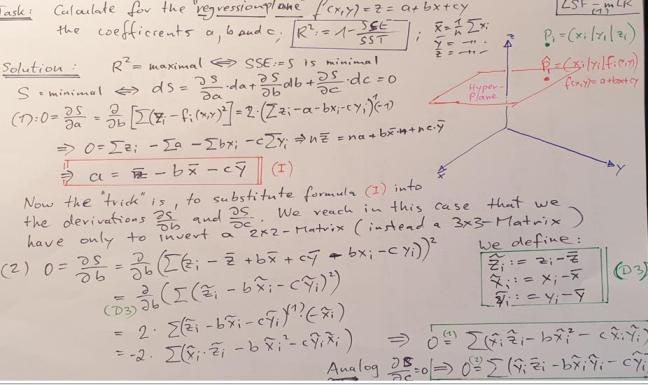
\includegraphics{LSF-mLR(k=2)-1}\\
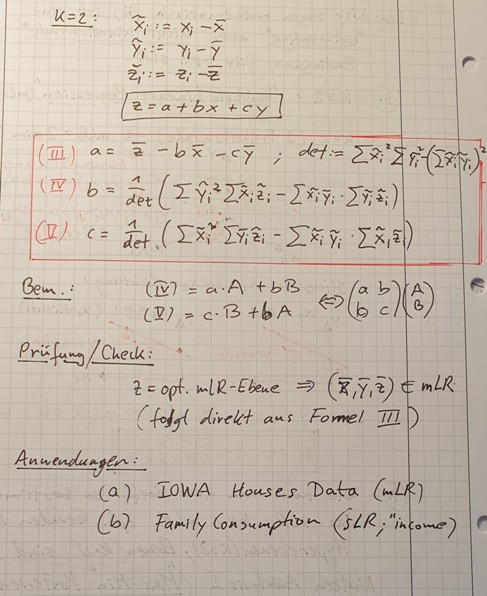
\includegraphics{LSF-mLR(k=2)-2}\\


*** Weitere Kapitel Texte ***

\subsection{simple Linear Regression (sLR) with Scikit-learn}

In order to get a better feeling for linear regression, we want to test it to investigate the factors that determine the fuel consumption of cars.  %\myFig{cars.csv} shows the head of the data file 
``\href{https://github.com/karlstroetmann/Artificial-Intelligence/blob/master/SetlX/cars.csv}{\texttt{cars.csv}}''
which I have adapted from the file
\\[0.2cm]
\hspace*{1.3cm}
\href{http://www-bcf.usc.edu/~gareth/ISL/Auto.csv}{\texttt{http://www-bcf.usc.edu/\symbol{126}gareth/ISL/Auto.csv}}.
\\[0.2cm]
%\myFig{cars.csv} shows the column headers and the first ten data entries contained in this file.  
Altogether, this file contains data of 392 different car models.
\\[0.1cm]
\hspace*{0.2cm}
\begin{center}
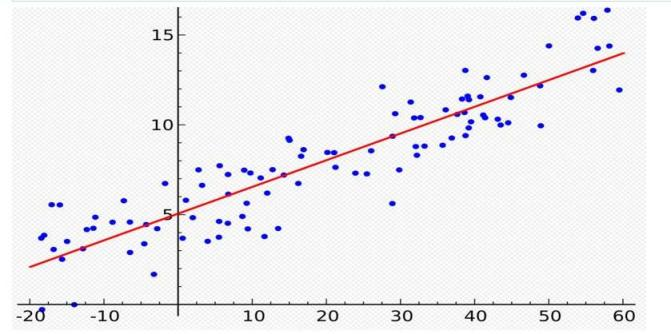
\includegraphics{sLR-Gerade} 
\end{center}

\subsection{Anwendungen zu mLR}

*** Weitere Kapitel Texte ***

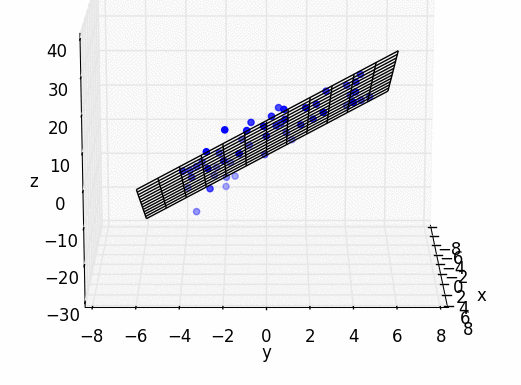
\includegraphics{ML5-MovingPicture_mLR}\\

Ein bewegtes Bild davon liegt in der Referenz [HVö-5]: 
\url{https://github.com/HVoellinger/Lecture-Notes-to-ML-WS2020/blob/master/ML5-QYuIc.gif}

\subsection{Übungen zum Kapitel 5}
{\color{red}
{*******************************************************************\\ 
ab hier bis Ende der Übungen sind die Folien der Vorlesung ML  zu nutzen und diese sind in Latex umzusetzen\\
********************************************************************\\}}



\subsubsection{Übung 5.1 - .......}
\begin{table}[h]
  \centering
  \begin{tabular}{|l|r|}
  \hline
  dependent variable      & explained variance   \\
  \hline
  \hline
  $\mathtt{displacement}$ & 0.75                 \\
  \hline
  $\mathtt{cyl}$          & 0.70                 \\
  \hline
  $\mathtt{hp}$           & 0.73                 \\
  \hline
  $\mathtt{weight}$       & 0.78                 \\
  \hline
  $\mathtt{acc}$          & 0.21                 \\
  \hline
  $\mathtt{year}$         & 0.31                 \\
  \hline
  \end{tabular}
  \caption[explained variance]{Explained variance for various dependent variables.}
  \label{tab:explained-variance}
\end{table}

\begin{table}[t] % Tabelle wird am oberen Rand der Seite platziert
  \centering
  \begin{tabular}{|c|c|}
    \hline
    Spalte 1 & Spalte 2 \\
    \hline
    Inhalt 1 & Inhalt 2 \\
    \hline
  \end{tabular}
  \caption{Eine Tabelle mit Positionsangabe "t".}
  \label{tab:tabelle_t}
\end{table}

% Weitere Tabellen mit anderen Positionsoptionen können hier folgen...



\subsubsection{Übung 5.2 - .......}


\begin{table}[h] % Tabelle wird hier eingefügt, wenn möglich
  \centering
  \begin{tabular}{|c|c|}
    \hline
    Spalte 1 & Spalte 2 \\
    \hline
    Inhalt 1 & Inhalt 2 \\
    \hline
  \end{tabular}
  \caption{Eine Tabelle mit Positionsangabe "h".}
  \label{tab:tabelle_h}
\end{table}


\subsubsection{Übung 5.3 - .......}
TEXT\\
\subsubsection{Übung 5.4 - .......}

\subsubsection{Übung 5.5}:

\textbf{Calculation of  mLR(k=2)-model for “Students Examination Results”}

Similar to Example (5.1): Find "least square fit" z = a + b*x + c*y for the z:=“Achieved points(score) of exam[pt.]” depending on the two parameter: x:="Effort exam preparation[h]" and y:=“Effort for homework [h]“. Data from Training Set TS  ={(x, y; z) | (exam prep.[h], homework[h]; score[pt.])}= {(7,5;41 ), (3,4;27), (5,5;35), (3,3;26), (8,9;48), (7,8;45), (10,10;46), (3,5;27), (5,3;29), (3,3;19)}
Task: Build to the model mLR(x,y; z). Compare and check your result with the output of a Python-Program.
Answer the following three Questions: 
Q1: How much points would a student achieve without any preparation and without doing any homework? 
Q2: How much points would a student achieve with (10 hours of preparation for the exam) and (10 hours homework) ? 
Q3: How much effort you will need to reach enough points (=25) to score enough points to pass the exam? 
Add. Question/Remark: Our calculation use both variables in the calculation. What is the difference to our sLR-model results? Compare Adj.R² (calculated here) to the two R² you got in Example (E5.1).

für eine Lösung vergleiche:\\
\url{https://github.com/HVoellinger/Lecture-Notes-to-ML-WS2020/blob/master/LR-Calculation_of_Coeff.xlsx}
\\

*** Weitere Kapitel Texte *** 

\newpage


\section{Text-Klassifikation mit dem Naive-Bayes-Klassifikator}


Wir zeigen hier Text-Klassifikation mit dem \textbf{Naive Bayes- Klassifikator} ("Bayes Learning" via "naïve Bayes Classifier"). Grundlage ist das Bayes-Theorem ("Bayes Rule"), welches sich mit bedingten Wahrscheinlichkeiten befasst.\\
Die Naive-Bayes-Textklassifikation ist eine Methode des maschinellen Lernens, die auf dem Naive-Bayes-Theorem basiert und häufig zur Kategorisierung von Textdaten verwendet wird. Sie ist besonders nützlich für Anwendungen wie Spam-Erkennung, Sentiment-Analyse, Themenklassifikation und mehr.\\

Der Ansatz ist "naiv", weil er eine starke Unabhängigkeitsannahme zwischen den Features (Wörtern) macht, was in der Praxis oft nicht der Fall ist.

\subsection{Eine Einführung in den naiven Bayes-Klassifikator}

Hier ist eine grundlegende Erklärung, wie die Naive-Bayes-Textklassifikation funktioniert:\\
\begin{figure}[htp]
  \centering
  \hspace*{-1.5cm} 
  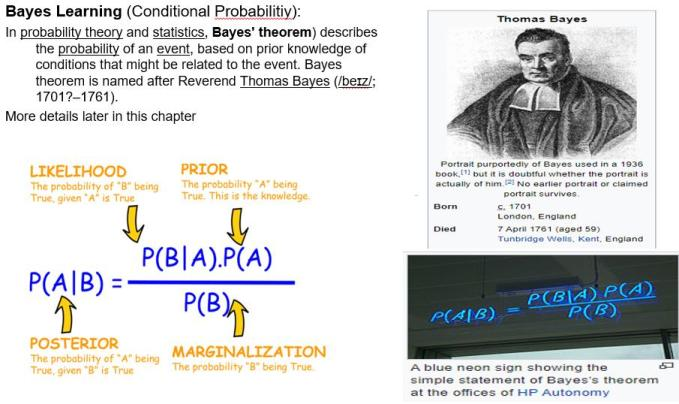
\includegraphics[width=1.2\textwidth]{Naive-Bayes-Learning}
  \caption{Screenshots zum Naive-Bayes-Learning}
\label{fig:NB_Learning}
\end{figure}


\textbf{1. Naive-Bayes-Theorem:}\\
Das Naive-Bayes-Theorem ist eine statistische Formel, die auf dem Satz von Wahrscheinlichkeitsregeln beruht, bekannt als \textbf{Bayes-Theorem}. Es gibt an, wie Wahrscheinlichkeiten nach der Anwendung neuer Informationen aktualisiert werden. Für die Textklassifikation bedeutet dies, dass wir die Wahrscheinlichkeit berechnen, mit der ein Dokument einer bestimmten Klasse (z. B. "Positiv" oder "Negativ") angehört, basierend auf den darin enthaltenen Wörtern.\\
\textbf{2. Feature-Extraktion:}\\
Für jeden Text werden Features (Wörter) extrahiert, die als Eingabe für den Naive-Bayes-Klassifikator dienen. In der Regel werden diese Wörter als "Bag of Words" betrachtet, d. h. die Reihenfolge der Wörter im Text wird ignoriert.\\
\textbf{3. Berechnung der Wahrscheinlichkeiten:}\\
Für jede Klasse wird die Wahrscheinlichkeit berechnet, dass ein gegebenes Dokument dieser Klasse angehört. Dies erfolgt, indem die Wahrscheinlichkeiten für jedes im Dokument vorkommende Wort (Feature) multipliziert werden. Die Wahrscheinlichkeiten werden aus Trainingsdaten abgeleitet.\\
\textbf{4. Klassifikation:}\\
Das Dokument wird der Klasse zugeordnet, für die die berechnete Wahrscheinlichkeit am höchsten ist. Dies wird oft durch den Satz von Klassenlabels erreicht, die im Trainingsprozess erlernt wurden.\\
\textbf{5. Laplace-Glättung:}\\
Ein Problem bei der Verwendung von Wahrscheinlichkeiten auf der Grundlage von Trainingsdaten ist, dass einige Wörter möglicherweise in bestimmten Klassen überhaupt nicht vorkommen. Dies könnte dazu führen, dass die berechnete Wahrscheinlichkeit null wird und das Modell nicht in der Lage ist, Vorhersagen für diese Klasse zu treffen. Um dieses Problem zu mildern, wird oft die Laplace-Glättung verwendet, um die Wahrscheinlichkeiten leicht zu verschieben.\\[0.2cm]

\textbf{Zusammenfassung:}\\
Naive-Bayes-Klassifikatoren sind einfach zu implementieren, schnell und können auch bei begrenzten Trainingsdaten gut funktionieren. Allerdings kann die starke Unabhängigkeitsannahme zwischen den Features in einigen Fällen zu weniger genauen Vorhersagen führen, insbesondere wenn es komplexe Abhängigkeiten zwischen den Wörtern gibt. Dennoch ist die Naive-Bayes-Textklassifikation eine nützliche Methode, um eine erste Annäherung an die Klassifikation von Textdaten zu erhalten.\\

\subsection{Mathematische Grundlagen bei Textklassifikatoren}
{\color{red}{*******************************************************************\\ 
ab hier bis Ende der section sind die Folien der Vorlesung ML  zu nutzen und diese sind in Latex umzusetzen\\
********************************************************************\\}}

\
\subsubsection{Bayes-Learning für Texte}

\begin{center} 
\hspace*{-1.5cm} 
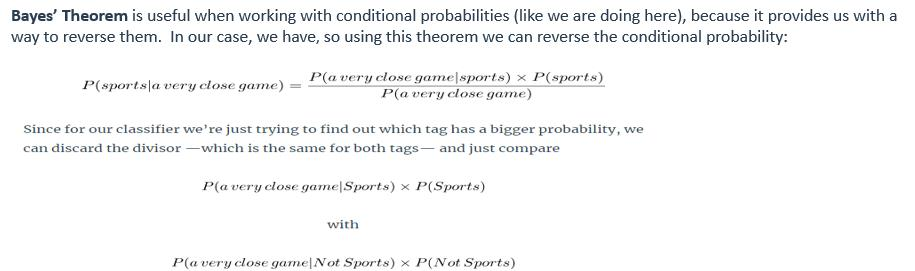
\includegraphics[width=1.2\textwidth]{Bayes-Rule01}
\end{center}

\subsubsection{"Laplace Glättung"}

\begin{center} 
\hspace*{-1.5cm} 
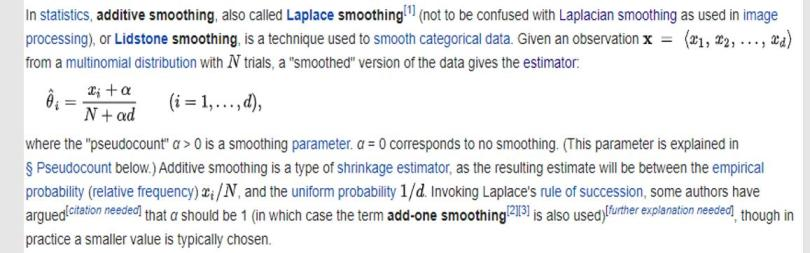
\includegraphics[width=1.2\textwidth]{Bayes-Rule02}
\end{center}

\subsection{Konkrete Anwendung des naiven Bayes-Klassifikator}

\begin{center}
\hspace*{-1.cm}   
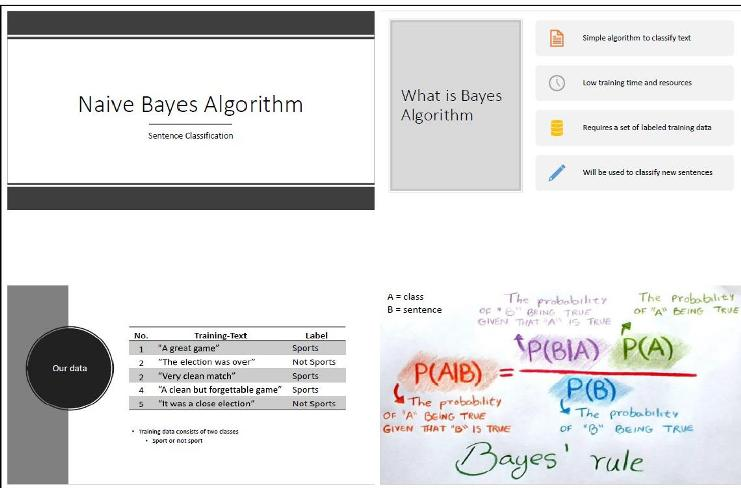
\includegraphics[width=1.2\textwidth]{Bayes-Text-Classification01}
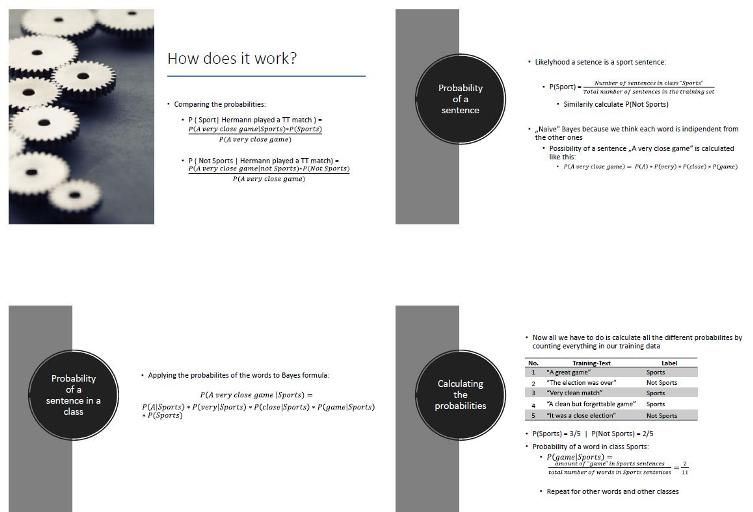
\includegraphics[width=1.1\textwidth]{Bayes-Text-Classification02}
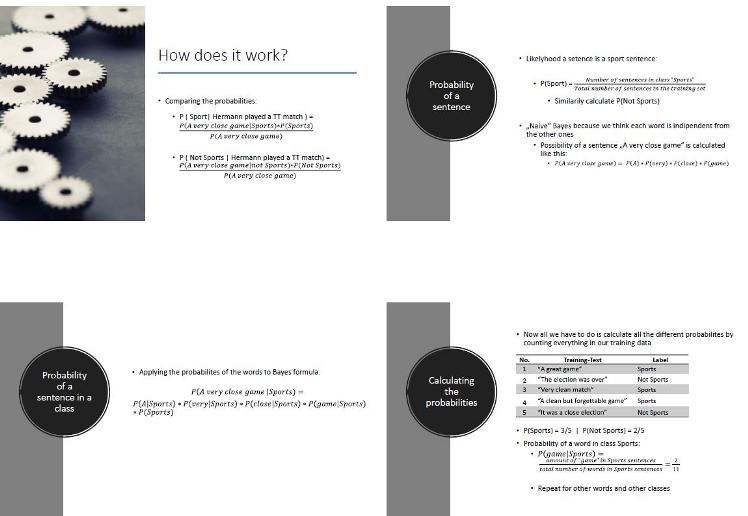
\includegraphics[width=1.1\textwidth]{Bayes-Text-Classification03}
\end{center}

\begin{center}  
\hspace*{-2.8cm} 
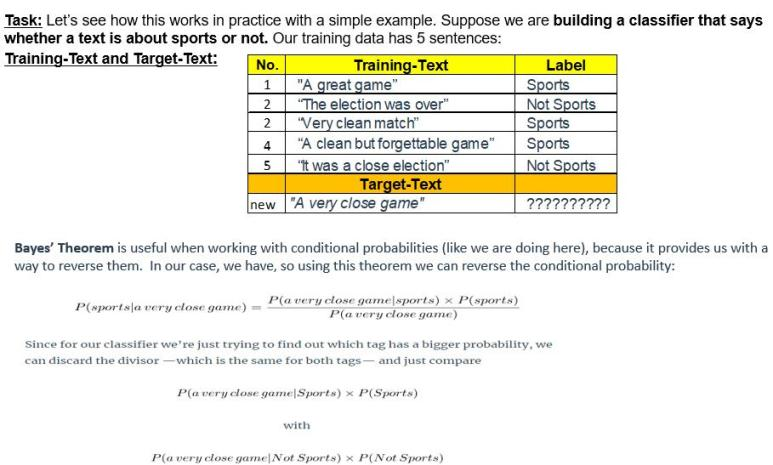
\includegraphics{Bayes-Beispiel01}
\end{center}

\begin{center}  
\hspace*{-2.5cm} 
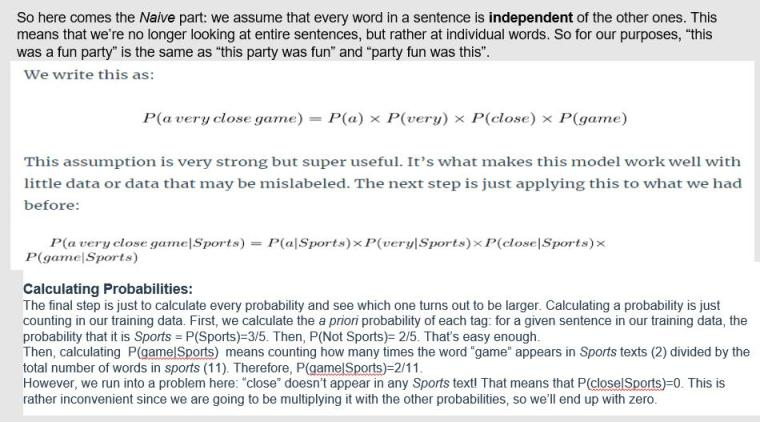
\includegraphics{Bayes-Beispiel02}
\end{center}\begin{center}  

\hspace*{-1.8cm} 
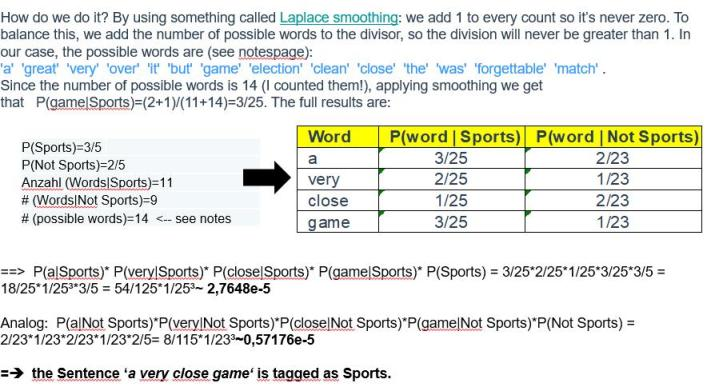
\includegraphics{Bayes-Beispiel03}
\end{center}

\newpage

\subsection{Übungen zum Kapitel 6}

{\color{red}{*******************************************************************\\ ab hier bis Ende der Übungen sind die Folien der Vorlesung ML  zu nutzen und diese sind in Latex umzusetzen\\
********************************************************************\\}}
.....\\



\subsubsection{Übung 6.1 - Bsp. einer Bayes-Texklassifikation}

Analog dem Beispiel aus obigen Kapitel soll die Bayes- Textklassifikation für einen weiteren Zielsatz mit den gleichen \textbf{"gelabelten" Trainingsdaten} durchgeführt werden. Wir suchen jetzt eine Klassifikation für den Zielsatz \textbf{"Hermann plays a TT match"}:\\   

\begin{center} 
\includegraphics[width=0.8\textwidth]{Bayes-Learning-Übungen}
\end{center}

\textbf{Zusatzfrage:} Wie verändert sich das Ergebnis wenn ich als Zielsatz: \textbf{"Hermann plays a very clean game"} eingebe? 


\subsubsection{Übung 6.2 - Bayes-Textklassifikation in Python}

Definiere einen Algorithmus in Python (benutze Jupyter Notebook) um obige Berechnung zu automatisieren. Tipp: Vergleich analoge Beispiele in \textbf{[HVö-5]} - \url{https://github.com/HVoellinger/Lecture-Notes-to-ML-WS2020}\\

\subsubsection{Übung 6.3}:
*** Weitere Kapitel Texte *** 

\newpage

\section{Verfahren der "Support Vector Machines" (SVM)}

*** Referenzen: [Wiki-SVM]; [SVM-Def] und  [TK + SVM]*****\\

Wichtig zum Verständnis von SVM ist die Beschreibung einiger mathematischen Grundlagen
der SVM. Diese sind in der Tat traditionelle Lineare Algebra und keine "Rocket Science". Es geht bei diesem Klassifikationsproblem darum optimale Hyperebenen zu finden die die Klassen "gut" trennen.
Dies kann man etwa auch gut am Beispiel von Text-Klassifikationen sehen. Text-Klassifikatiion hat sehr viel mit SVM zu tun. Vergleichen Sie dazu die Beispiele die in der Referenz [TK + SVM] zu sehen sind.
\subsection{Grundlegende mathematische Funktionsweise}
Das Hauptziel der SVM besteht darin, eine optimale Trennung (Klassifikation) zwischen zwei Klassen von Datenpunkten in einem mehrdimensionalen Raum zu finden. Die SVM sucht eine Hyperebene, die die beiden Klassen maximal voneinander trennt, wobei der Abstand zwischen der Hyperebene und den nächsten Datenpunkten (den sogenannten Support-Vektoren) maximiert wird.
\\
\textbf{Mathematisch Schreibweise:}
\\Angenommen, wir haben eine Menge von Trainingsdatenpunkten: ${(x_1, y_1), (x_2, y_2),... , (x_n, y_n)}$, wobei $x_i \in \mathbb{R}^n$ der Eingabevektor und $y_i$ als Klasse von Datenpunkten nur die Werte +1 oder -1 annehmen kann.\\
Für eine lineare SVM ist die mathematische Darstellung der Hyperebene dann gegeben durch:
\begin{center}
\begin{large} \textbf{$w \cdot x + b = 0$} \end{large} 
\end{center}
Hier ist "$w$" der Gewichtsvektor, der senkrecht zur Hyperebene zeigt und die Richtung der Trennung bestimmt. "$b$" ist der Bias (auch Verschiebungsparameter genannt), der die Verschiebung der Hyperebene entlang der "$w$"-Achse steuert. Es gelten dabei die folgenden \textbf{matematischen Bedingungen}\\
\textbf{1. Lineare Trennbarkeit:}\\
Die SVM hat bestimmte Trennbedingungen, die während des Trainingsprozesses erfüllt werden sollen:
Die Punkte jeder Klasse müssen auf unterschiedlichen Seiten der Hyperebene liegen.\\
Mathematisch ausgedrückt gilt für positive Beispiele ($y_i = 1$): $w \cdot x_i + b \geq 1$\\
und für negative Beispiele ($y_i = -1$): $w \cdot x_i + b \leq -1$\\
Der Abstand (Margin) zwischen den nächsten Datenpunkten (Support-Vektoren) und der Hyperebene muss maximal sein. Der Abstand zwischen zwei parallelen Hyperebenen, die die Support-Vektoren berühren, wird als Margin bezeichnet.\\
\textbf{2. Optimierung:}\\Das Ziel der SVM ist es, den Margin zu maximieren, indem die Länge des Gewichtsvektors "$w$" minimiert wird. Das führt zu einem quadratischen Optimierungsproblem. In der linearen SVM lautet das Optimierungsproblem:
\begin{center}
\begin{large} \textbf{Minimiere $||w||^2$} \end{large} \\
Unter den Bedingungen: $y_i \cdot (w \cdot x_i + b) \geq 1$ für alle Datenpunkte ${(x_i,y_i)}$
\end{center}
\textbf{3. Kernel-Trick:}\\
In Fällen, in denen die Daten nicht linear separierbar sind, kann der sogenannte Kernel-Trick angewendet werden. Der Kernel-Trick ermöglicht es, die Daten in einen höherdimensionalen Raum zu transformieren, in dem sie linear separierbar werden. Beliebte Kernel-Funktionen sind beispielsweise der lineare Kernel, der polynomiale Kernel und der RBF (Radial Basis Function) Kernel.\\

\textbf{Anmerkung: Wie kommt es zu dem Namen "Kernel-Trick"?}\\
Der Name "Kernel" kommt daher, dass in der mathematischen Darstellung der SVM die Funktion, die die Datenpunkte in den höherdimensionalen Raum transformiert, als Kernel-Funktion bezeichnet wird.\\

Dies sind die grundlegenden mathematischen Grundlagen der Support Vector Machine. SVM ist eine äußerst flexible und leistungsfähige Methode, die in vielen Anwendungen erfolgreich eingesetzt wird.\\

*** Weitere Kapitel Texte *** 

\subsection{Funktionsweise im Detail}

Ausgangsbasis für den Bau einer Support Vector Machine ist eine Menge von Trainingsobjekten, für die jeweils bekannt ist, welcher Klasse sie zugehören. Jedes Objekt wird durch einen Vektor in einem Vektorraum repräsentiert. Aufgabe der Support Vector Machine ist es, in diesen Raum eine Hyperebene einzupassen, die als Trennfläche fungiert und die Trainingsobjekte in zwei Klassen teilt. Der Abstand derjenigen Vektoren, die der Hyperebene am nächsten liegen, wird dabei maximiert. Dieser breite, leere Rand soll später dafür sorgen, dass auch Objekte, die nicht genau den Trainingsobjekten entsprechen, möglichst zuverlässig klassifiziert werden.
\begin{center} 
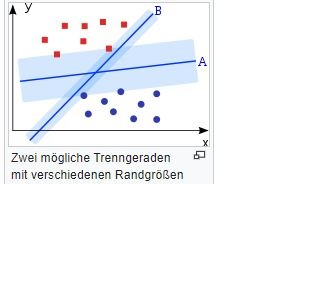
\includegraphics{SVM-Konzept} 
\end{center}
Beim Einsetzen der Hyperebene ist es nicht notwendig, alle Trainingsvektoren zu beachten. Vektoren, die weiter von der Hyperebene entfernt liegen und gewissermaßen hinter einer Front anderer Vektoren "versteckt" sind, beeinflussen Lage und Position der Trennebene nicht. Die Hyperebene ist nur von den ihr am nächsten liegenden Vektoren abhängig – und auch nur diese werden benötigt, um die Ebene mathematisch exakt zu beschreiben. Diese nächstliegenden Vektoren werden nach ihrer Funktion Stützvektoren (engl. support vectors) genannt und verhalfen den Support Vector Machines zu ihrem Namen.

\subsubsection{Lineare Trennbarkeit}

Eine Hyperebene kann nicht "verbogen" werden, sodass eine saubere Trennung mit einer Hyperebene nur dann möglich ist, wenn die Objekte linear trennbar sind.\\ 
\begin{center}  
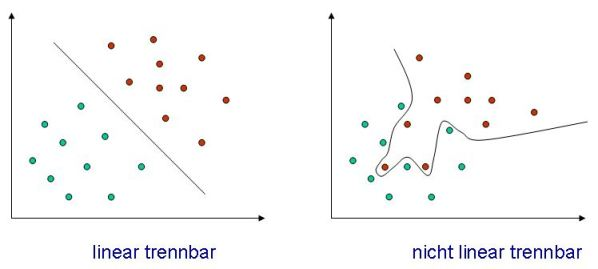
\includegraphics{Trennbarkeit}
\end{center}
Diese Bedingung ist für reale Trainingsobjektmengen im Allgemeinen nicht erfüllt. Support Vector Machines verwenden im Fall nichtlinear trennbarer Daten den \textbf{Kernel-Trick}, um eine nichtlineare Klassengrenze einzuziehen.\\

\subsubsection{Kernel-Trick}
Die Idee dahinter ist, den Vektorraum in einen höherdimensionalen Raum zu überführen, wo die Objekte linear trennbar sind und dort eine Hyperebene zu definieren. In einem Raum mit genügend hoher Dimensionsanzahl – im Zweifelsfall unendlich – wird auch die verschachtelteste Vektormenge linear trennbar. In diesem höherdimensionalen Raum wird nun die trennende Hyperebene bestimmt. Bei der Rücktransformation in den niedrigerdimensionalen Raum wird die lineare Hyperebene zu einer nichtlinearen, unter Umständen sogar nicht zusammenhängenden Hyperfläche, welche die Trainingsvektoren sauber in zwei Klassen trennt.\\
Bei diesem Vorgang stellen sich zwei Probleme: Die Hochtransformation ist enorm rechenintensiv und die Darstellung der Trennfläche im niedrigdimensionalen Raum im Allgemeinen unwahrscheinlich komplex und damit praktisch unbrauchbar. An dieser Stelle setzt der \textbf{Kernel-Trick} an. \\ Verwendet man zur Beschreibung der Trennfläche geeignete Kernelfunktionen, die im Hochdimensionalen die Hyperebene beschreiben und trotzdem im Niedrigdimensionalen "gutartig" bleiben, so ist es möglich, die Hin- und Rücktransformation umzusetzen, ohne sie tatsächlich rechnerisch ausführen zu müssen. Auch hier genügt ein Teil der Vektoren, nämlich wiederum die Stützvektoren, um die Klassengrenze vollständig zu beschreiben.\\
Sowohl lineare als auch nichtlineare Support Vector Machines lassen sich durch zusätzliche \textbf{Schlupfvariablen} flexibler gestalten. Die Schlupfvariablen erlauben es dem Klassifikator, einzelne Objekte falsch zu klassifizieren, "bestrafen" aber gleichzeitig jede derartige Fehleinordnung. Auf diese Weise wird zum einen Überanpassung vermieden, zum anderen wird die benötigte Anzahl an Stützvektoren gesenkt.

\subsection{Anschauliches 2-dim. Beispiel für Kernel-Trick}

Stellen wir uns ein einfaches und anschauliches Beispiel in $\mathbb{R}^2$ vor, bei dem die Datenpunkte im ursprünglichen Raum $(x_1,x_2)$ nicht linear trennbar sind.\\ 
Gesucht ist dann eine Abbildung $\Phi:\mathbb{R}^2 \rightarrow\mathbb{R}^3$, so das die Datenpunkte im höherdimensionalen Raum $(x,y,z)\in  \mathbb{R}^3$ linear trennbar sind.\\ 
Der Kernel-Trick ermöglicht es der SVM, die Entscheidungsgrenze in diesem höherdimensionalen Raum zu finden, ohne die zusätzlichen Merkmale $z$ tatsächlich berechnen zu müssen:\\ 
Gegeben sind die folgenden Datenpunkte: {\color{red}{Klasse +1: A(1,1), B(-1,1)}} und {\color{blue}{Klasse -1: C'(2,1), D(1,-2) und E(-2,1)}}.\\
In diesem Beispiel sind die Datenpunkte nicht linear trennbar (siehe auch nachfolgende Skizze). Es gibt keine gerade Linie, die die Punkte der {\color{red}{Klasse +1}} von den Punkten der {\color{blue}{Klasse -1}} perfekt trennen kann.\\
Jetzt wenden wir den Kernel-Trick an, um die Daten in $\mathbb{R}^3$ zu transformieren. Hier verwenden wir den polynomiellen Kernel über die folgende Transformation an: 
\begin{center}
 $\Phi:\mathbb{R}^2 \rightarrow\mathbb{R}^3$ definiert durch  $\Phi(x_1,x_2) = (x_1,x_2, x_1^2 + x_2^2)$. 
\end{center} 
Die transformierten Punkte A' = $\Phi(A)$ ....E' = $\Phi(A)$ werden dann berechnet als: {\color{red}{Klasse +1: A'(1,1,2), B'(-1,1,2)}} und {\color{blue}{Klasse -1: C'(2,1,5), D'(1,-2,5) und E'(-2,1,5)}}. Die roten Punkte liegen dabei alle auf der Höhe z=2 und die blauen Punkte auf z=5. Siehe dazu den folgenden Python Plot:\\[0.2cm]
\newpage
\begin{figure}[ht]
  \centering
  \hspace*{-0.5cm} 
  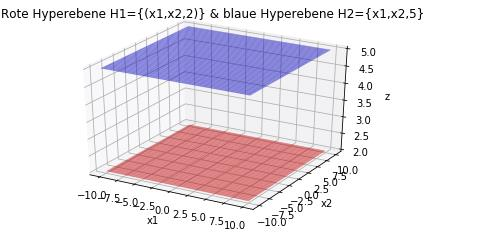
\includegraphics[width=0.9\textwidth]{Kernel-Hyperebene-Bild}
  \caption{Hyperebenen zum Kernel-Trick Beispiel}
  \label{fig:SVM_Ebenen}
\end{figure}

Ein bewegtes Bild davon liegt in der Referenz \textbf{[HVö-5]:} \url{https://github.com/HVoellinger/Mathematische-Grundlagen_von_ML/blob/main/Images/hyperebenen_animation.gif}\\[0.2cm]

Wie man leicht aus dem Plot sieht, lassen sich diese Punkte optimal durch eine Hyperebene ${H := \lbrace (x_1,x_2,z)| z=3,5\rbrace}$ trennen.\\ 
Durch eine "Zurücktransformation" erhält man den \textbf{Kreis: $x_1^2+x_2^2=3,5$ } mit den Radius $r = \sqrt[2]{3,5} \approx 1.871 $  Damit ergibt sich die visuelle Darstellung der Klassifikation-Trennlinie als Kreislinie. Wir lassen uns diesen Kreis via einem kleinem Python Programm ausploten:\\[0.2cm]
\begin{figure}[tp]
  \centering
  \hspace*{-0.1cm} 
  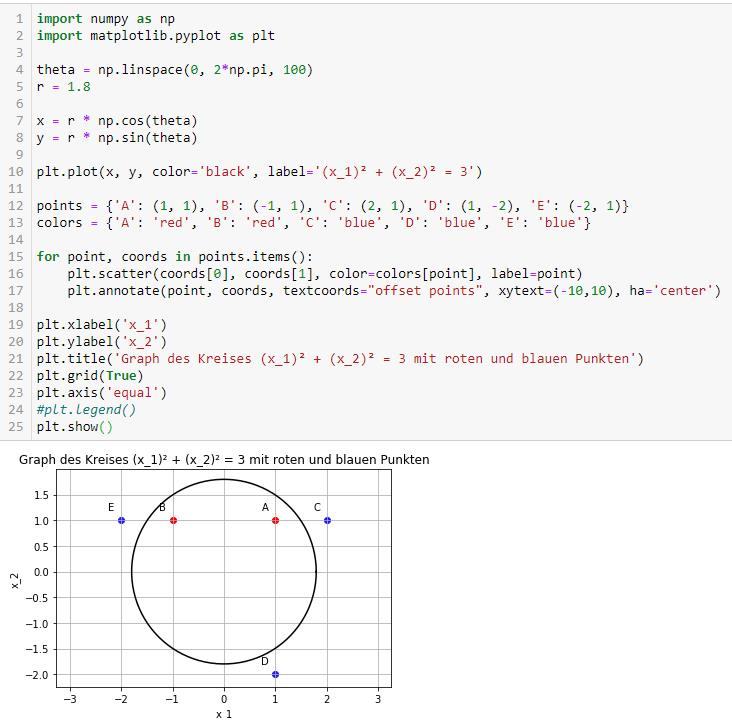
\includegraphics[width=1.1\textwidth]{SVM-Kreisbild-Python}
  \caption{Python Code und Kernel-Trick Kreisbild}       
  \label{fig:SVM_Kreis}
\end{figure}

\newpage

\subsection{Übungen zum Kapitel 7}



{\color{red}{*******************************************************************\\ 
ab hier bis Ende der Übungen sind die Folien der Vorlesung ML  zu nutzen und diese sind in Latex umzusetzen\\
********************************************************************\\}}
.....\\
\subsubsection{Übung 7.1 - .......}
TEXT\\
\subsubsection{Übung 7.2 - .......}

\subsubsection{Übung 7.3 - Python Code zu Hyperebenen}
Schreiben Sie den Python Code zur Generierung der zwei Hyperebenen im 2-dim. Beispiel zum Kernel-Trick. Animieren Sie die Grafik, so dass sie sich dreht. 

\newpage

\section{Neuronale Faltungsnetzwerke "Convolutional Neural Networks" (CNN)}

\textbf{Neuronale Faltungsnetzwerke} sind eine spezielle Art von künstlichen neuronalen Netzwerken, die hauptsächlich für die Verarbeitung von strukturierten Daten wie Bildern oder anderen Gitterdaten entwickelt wurden. Sie sind besonders effektiv bei der Extraktion von Merkmalen aus solchen Daten, was sie ideal für Aufgaben wie Bilderkennung und Bildklassifikation macht.
\\
Der Name "Faltungsnetzwerke" leitet sich von der \textbf{Faltungsoperation} ab, die in diesen Netzwerken eine wichtige Rolle spielt. Diese Operation ermöglicht es, lokale Merkmale oder Muster in den Eingabedaten zu erkennen, indem sie über die Daten "geschoben" wird. Diese Merkmale werden dann auf höheren Ebenen des Netzwerks kombiniert, um komplexere Muster und Strukturen zu identifizieren.
\\Convolutional Neural Networks (CNNs) sind eine spezielle Art von \textbf {Deep-Learning-Modellen}. Insgesamt bezieht sich "Deep Learning" auf den Einsatz von neuronalen Netzwerken mit mehreren Schichten (daher "tief") für das Lernen von Darstellungen und Mustern in Daten. CNNs sind nur eine von vielen Architekturen im Bereich des Deep Learning.\\
CNNs haben in den letzten Jahren große Fortschritte erzielt und sind zum Beispiel in der Bilderkennung, Gesichtserkennung, medizinischen Bildverarbeitung und sogar in der natürlichen Sprachverarbeitung (mit Modellen wie den sogenannten "Convolutional Seq2Seq" Modellen) weit verbreitet.\\
***\\
***\\ Weitere Kapitel Texte \\
***\\
**** Referenz: [Math for DL] ******** 
\subsection{Mathematische Grundlagen von CNN}
Die mathematischen Grundlagen des Convolutional Neural Networks (CNN) beruhen auf Konzepten aus linearen Algebra, partiellen Ableitungen und Faltung (Convolution). Ein CNN ist eine spezielle Art von neuronalem Netzwerk, das häufig in der Bild- und Sprachverarbeitung eingesetzt wird, aufgrund seiner Fähigkeit, räumliche Strukturen in Daten zu erkennen.\\
Hier sind die wichtigen mathematischen Grundlagen eines Convolutional Neural Networks:\\

\textbf{1. Lineare Algebra:}\\
CNNs verwenden Matrizenoperationen, um Gewichte und Aktivierungen zu berechnen. Ein typischer Schritt in einem CNN ist die lineare Transformation, bei der Eingabedaten durch eine Gewichtsmatrix multipliziert und ein Bias addiert wird. Dies erzeugt die Aktivierungen der nächsten Schicht.\\
\textbf{2. Faltung (Convolution):}\\
Die Faltung ist ein zentrales Konzept in CNNs. In einem CNN werden Filter (auch Kernel genannt) verwendet, um räumliche Merkmale aus den Eingabedaten zu extrahieren. Die Faltung erfolgt durch das Verschieben des Filters über die Eingabedaten und die Berechnung des Punktprodukts zwischen dem Filter und dem überlappenden Teil der Daten. Das Ergebnis ist ein sogenanntes Aktivierungsmuster oder Feature-Map, das die erkannten Merkmale anzeigt.\\
\textbf{3. Nichtlinearität (Aktivierungsfunktionen):}\\
Nach der Faltung wird in den meisten Schichten des CNN eine Nichtlinearität eingeführt, um die Expressivität des Netzwerks zu erhöhen. Eine Aktivierungsfunktion wie die ReLU (Rectified Linear Unit) wird oft verwendet, um negative Werte zu eliminieren und nichtlineare Verzerrungen in den Daten zu erzeugen.\\
\textbf{4. Pooling:}\\
Pooling ist ein weiterer wichtiger Schritt in CNNs, um die räumliche Dimension der Daten zu reduzieren und die Invarianz gegenüber leichten Translationen zu erreichen. Typischerweise wird Max-Pooling angewendet, bei dem der maximalste Wert aus einem kleinen Ausschnitt der Daten beibehalten wird.\\
\textbf{5. Backpropagation:}\\
Wie bei anderen neuronalen Netzwerken werden CNNs mit dem Backpropagation-Algorithmus trainiert. Backpropagation verwendet die Kettenregel der partiellen Ableitungen, um die Gewichte des Netzwerks so anzupassen, dass der Fehler zwischen den vorhergesagten und tatsächlichen Ausgaben minimiert wird.\\
\textbf{6. Mehrschichtige Struktur:}\\
CNNs bestehen aus mehreren Schichten, darunter Eingabeschicht, Faltungsschichten, Aktivierungsschichten, Pooling-Schichten und einer Ausgabeschicht. Die tieferen Schichten sind in der Lage, einfache Merkmale zu lernen, während die höheren Schichten komplexere Merkmale und Kombinationen von Merkmalen erfassen können.
\\
Diese mathematischen Grundlagen ermöglichen es Convolutional Neural Networks, Merkmale aus Eingabedaten zu extrahieren und komplexe Muster zu lernen, was zu einer effektiven Verarbeitung von Bildern, Videos, Sprache und anderen räumlichen Daten führt.

\subsection{Rückwärtspropagierung für ein anschauliches Beispiel}

Die Rückwärtspropagierung ("Backpropagation") erfolgt um die Gewichte zu aktualisieren und den Fehler zu minimieren. Durch diese Schritte werden die Gewichte des neuronalen Netzwerks iterativ angepasst, um den \textbf{Fehler zwischen den vorhergesagten und tatsächlichen Ausgaben zu minimieren} und bessere Vorhersagen zu machen. Der Vorgang wird für jeden Eingabedatensatz und seine zugehörige Ausgabe wiederholt, bis das Netzwerk trainiert ist.
\\Lassen Sie uns einfaches Beispiel für den Backpropagation-Prozess für ein sehr einfaches neuronales Netz mit nur einer versteckten Schicht ("Hidden Layer") durchgehen. Insgesamt haben ein neuronales Netzwerk mit zwei Eingängen, zwei versteckten Neuronen und zwei Ausgangsneuronen. Zusätzlich werden die versteckten Neuronen und die Ausgangsneuronen einen Bias (aka: Verzerrungen") enthalten. An diesem 3-Schichten CNN können wir den kompletten Backpropagation Prozess beispielhaft berechnen:\\
\textbf{Eingabeschicht ("Input Layer" mit 2 "Input Nodes" $(i_1,i_2)$) $\Rightarrow$ Verarbeitunsschicht ("Hidden Layer" mit 2 "Hidden Nodes "$(h_1,h_2)$ ) $\Rightarrow$ Ausgabeschicht ("Output Layer" mit 2 "Output Nodes" $(o_1,o_2)$).} \\ 
Um ein paar Zahlen zu haben, mit denen man arbeiten kann, sind hier die {\color{red}{anfänglichen Gewichte}}, die {\color{orange}{Bias("Verzerrungen")}} und die {\color{blue}{Trainingsinputs/-outputs}} angegeben:\\

\begin{center}
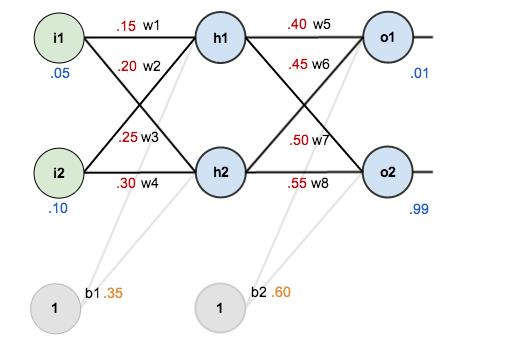
\includegraphics{Backpropagation_Example3} 
\end{center}

\subsubsection{Berechnungen zum Vorwärtsdurchlauf ("Forward Pass")}
Der Vorwärtsdurchlauf (englisch: forward pass) bei Convolutional Neural Networks (CNNs) ist der Prozess, bei dem die Eingabedaten durch das Netzwerk propagiert werden, um eine Vorhersage oder Ausgabe zu generieren. Während des Vorwärtsdurchlaufs werden die Daten Schicht für Schicht verarbeitet, wobei die Gewichtungen, Aktivierungen und Pooling-Operationen angewendet werden, um schließlich die Ausgabe zu erhalten.\\
Berechnen wir zunächst die gewichtete Summe ($h_1, h_2$) und glätten dann den  Wertebereich durch die \textbf{logistische Funktion} $\sigma(z) := \frac{1}{1 + e^{-z}}$) (siehe auch die Anmerkung dazu weiter unten im Text) um die Ausgaben der versteckten Schicht zu erhalten.\\ Wir bezeichne diese mit Großbuchstaben $(H_1,H_2)$:
\\ 
\[
\begin{aligned}
h_1 &= (i_1 \cdot w_1) + (i_2 \cdot w_2) + b_1 = (0.05 \cdot 0.15) + (0.1 \cdot 0.25) + 0.35 = 0.3775 \\
h_2 &= (i_1 \cdot w_3) + (i_2 \cdot w_4) + b_1 = (0.05 \cdot 0.2) + (0.1 \cdot 0.3) + 0.35 = 0.3925\\
H_1 &= \sigma(h_1) = \frac{1}{1 + e^{-0.3775}} \approx 0.5933 \\
H_2 &= \sigma(h_2) = \frac{1}{1 + e^{-0.3925}} \approx 0.5969 \\
\end{aligned}\]
Wir wiederholen diesen Vorgang für die Neuronen der Ausgabeschicht und verwenden die Ausgaben der Neuronen der versteckten Schicht als Eingaben. Wir bezeichnen die Ergebnisse Ausgabeschicht mit Großbuchstaben $(O_1,O_2)$:$(i_1,i_2)$\\
\[
\begin{aligned}
o_1 &= (a_1 \cdot w_5) + (a_2 \cdot w_6) + b_2 = (0.5933 \cdot 0.4) + (0.5969 \cdot 0.45) + 0.6 \approx 1.1059 \\
O_1 &= \sigma(o_1) \approx 0.7514\\
o_2 &= (a_1 \cdot w_7) + (a_2 \cdot w_8) + b_2 = (0.5933 \cdot 0.5) + (0.5969 \cdot 0.55) + 0.6 \approx 1.2249 \\
O_2 &= \sigma(o_2) \approx 0.7729\\
\end{aligned}
\]
\\
\textbf{Anmerkung zur "logistischen Funktion":}
\\Die Sigmoid-Funktion $\sigma(z)$ glättet den Wertebereich und ist aufgrund ihres kontinuierlichen Verlaufs gut für die Berechnung von Gradienten bei der Rückwärtspropagation (Backpropagation) geeignet. Sie wird in CNNs und anderen neuronalen Netzwerken häufig verwendet, um die Aktivierungsstärke eines Neurons zu modulieren.\\
Die Sigmoid-Funktion ist eine nichtlineare Funktion, die eine kontinuierliche Ausgabe zwischen 0 und 1 erzeugt. Der folgende Graph zeigt den S-förmigen Verlauf der logistischen Funktion  $\sigma(z)$ über den Bereich von z=-6 bis z=+6:\\
\begin{center}
\begin{tikzpicture}
\begin{axis}[
    xlabel=$z$,
    ylabel={$\sigma(z)$},
    axis lines=middle,
    ymin=-0.1, ymax=1.1,
    xmin=-6, xmax=6,
    xtick={-5,-4,-3,-2,-1,0,1,2,3,4,5},
    ytick={0,0.2,0.4,0.6,0.8,1},
    xticklabels={$-5$,$-4$,$-3$,$-2$,$-1$,$0$,$1$,$2$,$3$,$4$,$5$},
    yticklabels={$0$,$0.2$,$0.4$,$0.6$,$0.8$,$1$},
    samples=100,
    smooth
]
\addplot[blue, domain=-6:6] {1 / (1 + exp(-x))};
\end{axis}
\end{tikzpicture}
\end{center}
\textbf{Bemerkung}: Die Sigmoid-Aktivierung wurde früher häufiger verwendet, hat jedoch in einigen Situationen Probleme wie das Verschwinden von Gradienten verursacht. Aus diesem Grund verwenden moderne CNN-Architekturen oft ReLU (Rectified Linear Unit) und ihre Varianten als Aktivierungsfunktionen, da sie das Problem des Verschwindens von Gradienten verringern und zur schnelleren Konvergenz des Lernprozesses beitragen können.

\subsubsection{Berechnungen des Fehlers/Verlustes "Error/Loss":}

Wir können nun den Fehler für jedes Ausgangsneuron mit Hilfe der quadratischen Fehlerfunktion berechnen und sie addieren, um den Gesamtfehler zu erhalten.\\
Anmerkung: Die $\frac{1}{2}$ ist enthalten, damit der Exponent beim späteren Differenzieren aufgehoben wird. Das Ergebnis wird schließlich ohnehin mit einer Lernrate $\eta$ multipliziert, so dass es keine Rolle spielt, dass wir hier eine Konstante einführen. \\ Bezeichne den Fehler ("Error") pro Ausgabeneuron wieder mit Großbuchstaben $(E_1,E_2)$ und den Gesamtfehler als $E$, so ergibt sich: 
\[ 
\begin{aligned}
E_1 &= \frac{1}{2} \cdot (b_1 - y_{\text{target1}})^2 \approx \frac{1}{2} \cdot (0.7514 - 0.01)^2 \approx 0.2748
\\
E_2 &= \frac{1}{2} \cdot (b_2 - y_{\text{target2}})^2 \approx \frac{1}{2} \cdot (0.7729 - 0.99)^2 \approx 0.0236 
\\
E &= E_1 + E_2 \approx 0.2748 + 0.0236 \approx 0.2983
\end{aligned} 
\]
\\
\subsubsection{Rückwärtsdurchlauf "Backward Pass":}
Unser Ziel bei der Backpropagation ist es, die einzelnen Gewichte im Netz so zu aktualisieren, dass die tatsächliche Ausgabe näher an der Zielausgabe liegt, wodurch der Fehler für jedes Ausgangsneuron und das Netz als Ganzes minimiert wird.\\
In der nachfolgenden Grafik ist das Vorgehen schematisch dargestellt. Insbesondere kommt die \textbf{Kettenregel von "geschachtelten" Funktionen} zur Anwendung (siehe Vorlesung "Analysis I + II"):

\begin{figure}[htb]
  \centering
  \vspace*{0.5cm}
 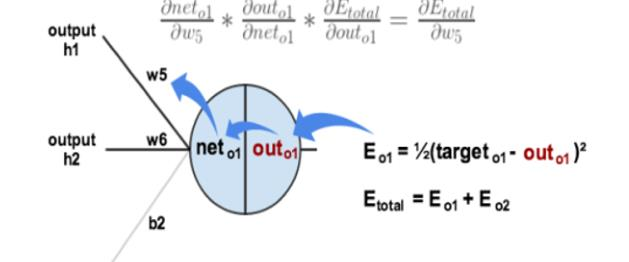
\includegraphics{Backpropagation-BP} 
  \vspace*{-0.5cm}
  \caption{Backpropagation-Rückwärtslauf}
\end{figure}
{\color{red}{*******************************************************************\\ ******* ab hier bis Ende subsection ist dass noch anzupassen ******* \\
********************************************************************\\}}
\[
\begin{aligned}
\frac{\partial \text{loss}}{\partial a_3} &= a_3 - y_{\text{target}} \approx 0.6685 - 1 \approx -0.3315 \\
\frac{\partial a_3}{\partial z_3} &= a_3 \cdot (1 - a_3) \approx 0.6685 \cdot (1 - 0.6685) \approx 0.2241 \\
\frac{\partial \text{loss}}{\partial w_5} &= \frac{\partial \text{loss}}{\partial a_3} \cdot \frac{\partial a_3}{\partial z_3} \cdot a_1 \approx -0.3315 \cdot 0.2241 \cdot 0.6682 \approx -0.0664 \\
\frac{\partial \text{loss}}{\partial w_6} &= \frac{\partial \text{loss}}{\partial a_3} \cdot \frac{\partial a_3}{\partial z_3} \cdot a_2 \approx -0.3315 \cdot 0.2241 \cdot 0.8909 \approx -0.0497 \\
\frac{\partial \text{loss}}{\partial b_3} &= \frac{\partial \text{loss}}{\partial a_3} \cdot \frac{\partial a_3}{\partial z_3} \approx -0.3315 \cdot 0.2241 \approx -0.0743 \\
\end{aligned}
\] \\[0.2cm]

Wir multiplizieren die Gewichte $w_i$ und die Biases $b_i$ mit einer Lernrate (e.g., $\eta = 0.1$):\\

\[
\begin{aligned}
w_5' &= w_5 - \eta \cdot \frac{\partial \text{loss}}{\partial w_5} \approx 0.2 - 0.1 \cdot (-0.0664) \approx 0.3066 \\
w_6' &= w_6 - \eta \cdot \frac{\partial \text{loss}}{\partial w_6} \approx 0.4 - 0.1 \cdot (-0.0497) \approx 0.7050 \\
b_3' &= b_3 - \eta \cdot \frac{\partial \text{loss}}{\partial b_3} \approx 0.1 - 0.1 \cdot (-0.0743) \approx 0.2074 \\
\end{aligned}
\]

In ähnlicher Weise werden die Gradienten berechnet und die Gewichte und Verzerrungen für die Verbindungen zwischen der Eingabeschicht und der verborgenen Schicht aktualisiert.

Dieser Prozess des Vorwärtsdurchlaufs, der Verlustberechnung und des Rückwärtsdurchlaufs wird iterativ über den gesamten Trainingsdatensatz wiederholt, um die Gewichte und Verzerrungen zu aktualisieren, bis das Netzwerk lernt, genaue Vorhersagen zu treffen.\\[0.2cm]

Weitere Details unter folgenden \textbf{Referenzen:} [BackP-Exam] und [BackP-Scikit]  
\newpage

\subsection{Übungen zum Kapitel 8}

{\color{red}{*******************************************************************\\ 
ab hier bis Ende der Übungen sind die Folien der Vorlesung ML  zu nutzen und diese sind in Latex umzusetzen\\
********************************************************************\\}}  
.....\\
\subsubsection{Übung 8.1 - CNN Architekur}
TEXT\\
\subsubsection{Übung 8.2 - Beispiel Backpropagation}
.....\\
\subsubsection{Übung 8.3 - ...............}

\newpage


\section{Anhänge}

In den Anhängen werden einige weitere Verfahren des Maschinellen Lernens der Vollständigkeit halber erwähnt - ohne zu sehr in die inhaltlich Tiefe zu gehen. Zukünftig können jedoch diesem Themen in einer erweiterten Version des Skriptes durchaus nochmals aufgegriffen werden.  \\[0.2cm]


\subsection{Empfehlungssysteme "Recommender Systems" (LinAlgebra)}
Die mathematischen Grundlagen von Recommender Systems (auch als Empfehlungssysteme bezeichnet) hängen von der spezifischen Art des Empfehlungssystems ab. Es gibt verschiedene Ansätze und Modelle, die in Recommender Systems verwendet werden, um Empfehlungen für Benutzer zu generieren.\\
Hier sind einige der wichtigsten mathematischen Grundlagen:\\

\textbf{1. Collaborative Filtering (Kollaborative Filterung):} Bei der kollaborativen Filterung werden Empfehlungen basierend auf der Ähnlichkeit zwischen Benutzern oder Objekten generiert. Diese Ähnlichkeit kann durch Berechnung von Ähnlichkeitsmetriken wie der Kosinusähnlichkeit oder der Pearson-Korrelation zwischen Benutzern oder Objekten ermittelt werden.\\

\textbf{2. Matrix Factorization (Matrizenfaktorisierung):} Dies ist eine Technik, bei der die Bewertungen von Benutzern für Objekte in eine niedrigdimensionale latente Raum eingebettet werden. Diese Einbettung ermöglicht es, die Bewertungen als Produkte von latenten Benutzer- und Objektvektoren darzustellen. Die Matrix wird in zwei niedrigdimensionale Matrizen (Benutzermatrix und Objektmatrix) zerlegt, und Empfehlungen werden basierend auf den latenten Vektoren berechnet.\\

\textbf{3. Content-Based Filtering (Inhaltsbasierte Filterung):} Hier werden Empfehlungen basierend auf den Merkmalen (Eigenschaften) der Objekte und den Präferenzen der Benutzer generiert. Ähnlichkeiten zwischen Objekten werden durch Ähnlichkeitsmaße wie den Kosinusähnlichkeitswert der Merkmale berechnet.\\
\textbf{4. Singular Value Decomposition (SVD):} SVD ist eine Technik der linearen Algebra, die zur Dimensionsreduktion und Matrizenfaktorisierung verwendet wird. Im Zusammenhang mit Recommender Systems wird SVD häufig in der Matrixfaktorisierung für kollaborative Filterung angewendet.\\

\textbf{5. ** Deep Learning **:} In den letzten Jahren haben Recommender Systems auch von den Fortschritten im Bereich des Deep Learning profitiert. Hier werden neuronale Netzwerke verwendet, um komplexe Muster in den Daten zu lernen und präzisere Empfehlungen zu generieren.\\

\textbf{6. Evaluation Metrics (Auswertungsmetriken):} Um die Leistung von Recommender Systems zu bewerten, werden verschiedene Auswertungsmetriken verwendet, wie zum Beispiel Genauigkeit, Trefferquote, Mittlere absolute Fehler (MAE) oder Mittlere quadratische Abweichung (MSE).\\[0.2cm]

\textbf{Zusammenfassung:} Je nach Art des Recommender Systems können weitere mathematische Konzepte und Modelle involviert sein. Die Grundlagen der Mathematik und Statistik spielen jedoch eine entscheidende Rolle bei der Modellierung, Berechnung und Bewertung von Empfehlungssystemen, um nützliche und relevante Empfehlungen für die Benutzer zu generieren.\\


\newpage

\subsection{Regularisierungen und Lineare Algebra (LA)}

\subsubsection{Regularisierung in maschinellem Lernen}
Regularisierung ist eine Technik im maschinellen Lernen, die verwendet wird, um Overfitting zu vermeiden. Overfitting tritt auf, wenn ein Modell zu stark auf die Trainingsdaten passt und dadurch auf neuen, bisher ungesehenen Daten schlecht abschneidet. Regularisierung fügt eine zusätzliche Bedingung zur Verlustfunktion hinzu, um die Gewichtungen im Modell zu begrenzen oder einzuschränken.

Es gibt zwei gängige Arten von Regularisierung:\\

1. \textbf{L2-Regularisierung (Ridge-Regularisierung)}: Hierbei wird der Verlustfunktion ein Ausdruck hinzugefügt, der proportional zur Quadratsumme der Gewichtungen ist. Dies zwingt das Modell dazu, die Gewichtungen kleiner zu halten.\\

2. \textbf{L1-Regularisierung (Lasso-Regularisierung)}: Bei dieser Methode wird der Verlustfunktion ein Ausdruck hinzugefügt, der proportional zur Summe der absoluten Werte der Gewichtungen ist. Dadurch neigen viele der Gewichtungen im Modell dazu, genau null zu werden, was zu einer Art von Feature-Auswahl führt.\\

\subsubsection{Lineare Algebra in Bezug auf Regularisierung}
Lineare Algebra ist ein wichtiger Teilbereich der Mathematik, der sich mit Vektoren, Matrizen und linearen Gleichungssystemen befasst. Sie spielt eine bedeutende Rolle in der Vorstellung und Berechnung von Regularisierungstechniken. Hier sind einige Punkte, wie Lineare Algebra mit Regularisierung zusammenhängt:\\

1. \textbf{Gewichtungen als Vektoren:} In maschinellen Lernalgorithmen werden die Gewichtungen oft als Vektoren dargestellt. Diese Vektoren werden mithilfe von Linearer Algebra manipuliert, um die Regularisierungsbedingungen zu erfüllen.\\

2. \textbf{Matrixformulierung:} Viele Regularisierungstechniken können in der Matrixformulierung ausgedrückt werden. Zum Beispiel kann die L2-Regularisierung als Hinzufügen eines Ausdrucks zur Verlustfunktion betrachtet werden, der mit der Quadratwurzel der Gewichtungsmatrix multipliziert wird.\\

3. \textbf{Optimierung:} Bei der Anwendung von Regularisierungstechniken wird häufig eine Verlustfunktion optimiert, um die besten Gewichtungen zu finden. Lineare Algebra spielt eine Rolle bei der Ableitung und Lösung dieser Optimierungsprobleme.\\

4. \textbf{Eigenschaften von Matrizen:} In einigen Fällen können Eigenschaften von Matrizen genutzt werden, um Regularisierungsverfahren zu analysieren und zu verstehen.\\[0.15cm]

Insgesamt ist die \textbf{Lineare Algebra} ein unverzichtbares Werkzeug, wenn es darum geht, Regularisierung in maschinellem Lernen zu verstehen, zu implementieren und anzuwenden. Sie ermöglicht es, die mathematischen Grundlagen hinter diesen Techniken zu verstehen und effektiv mit komplexen Modellen zu arbeiten. \\

\newpage

\subsection{Hauptkomponentenanalyse "Principal Component Analysis" (PCA)}
 
Die Hauptkomponentenanalyse (Englisch: "Principal Component Analysis") kurz: PCA) ist auch als Hauptachsentransformation bekannt. Das PCA  ein Verfahren der multivariaten Statistik.\\
Sie strukturiert umfangreiche Datensätze durch Benutzung der Eigenvektoren der Kovarianzmatrix. Dadurch können Datensätze vereinfacht und veranschaulicht werden, indem eine Vielzahl statistischer Variablen durch eine geringere Zahl möglichst aussagekräftiger Linearkombinationen (die Hauptkomponenten) genähert wird.\\
Speziell in der Bildverarbeitung wird die Hauptkomponentenanalyse, auch \textit{Karhunen-Loève-Transformation} genannt, benutzt. Sie ist von der Faktoren-Analyse zu unterscheiden, mit der sie formale Ähnlichkeit hat und in der sie als Näherungsmethode zur Faktorenextraktion verwendet werden kann (der Unterschied der beiden Verfahren kann in Wikipedia nachgelesen werden). \\[0.2cm]
\begin{figure}[h]
  \centering
  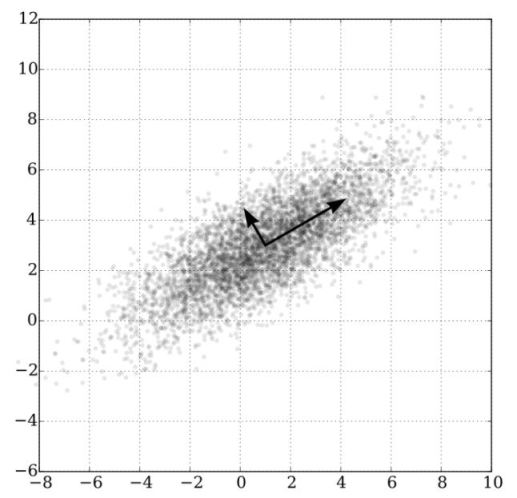
\includegraphics[width=0.6
  \textwidth]{Hauptkomponentenanalyse}
  \caption{Schematische Darstellung der Hauptkomponentenanalyse}
  \label{fig:HK_A}
\end{figure}
Das Bild unten zeigt die \textbf{Hauptkomponentenanalyse als Faktorenanalyse}.\\ Zwei Hauptkomponenten einer zweidimensionalen Normalverteilung mit Mittelwert (1,3) und Standardabweichung circa 3 in (0.866, 0.5)-Richtung und 1 in die dazu orthogonale Richtung. Die Vektoren sind die Eigenvektoren der Kovarianzmatrix und haben als Länge die Wurzel des zugehörigen Eigenwertes. Sie sind so verschoben, dass sie am Mittelwert ansetzen. \\[0.2cm]
Es gibt verschiedene \textbf{Verallgemeinerungen} der Hauptkomponentenanalyse, z. B. die Hauptkurven ("Principal Curves"), die Hauptflächen ("Principal Surfaces"), t-verteilte stochastische Nachbarschaftseinbettung ("t-distributed stochastic neighbor embedding") oder die kernbasierte Hauptkomponentenanalyse ("kernel Principal Component Analysis", kurz: kernel PCA).\\

\newpage


\subsection{Singulärwertzerlegung "Singular Value Decomposition" (SVD)}

Eine \textbf{Singulärwertzerlegung} (engl. Singular Value Decomposition; abgekürzt SWZ oder SVD) einer Matrix bezeichnet deren Darstellung als Produkt dreier spezieller Matrizen. Daraus kann man die Singulärwerte der Matrix ablesen. Diese charakterisieren, ähnlich den Eigenwerten, Eigenschaften der Matrix. Singulärwertzerlegungen existieren für jede Matrix – auch für nichtquadratische Matrizen.\\
\textbf{Singulärwertzerlegung am Beispiel einer zweidimensionalen, reellen Scherung M}: Diese Transformation verzerrt den blauen Einheitskreis oben links zur Ellipse rechts oben im Bild. M kann zerlegt werden in zwei Drehungen U und V* sowie eine Dehnung/Stauchung $\Sigma$  entlang der Koordinatenachsen. Die Singulärwerte $\sigma1$ und $\sigma2$ sind die Längen der großen bzw. kleinen Halbachse der Ellipse.\\ 
 
\begin{figure}[htb]
  \centering
  \includegraphics[width=0.6\textwidth]{Singulärwertszerlegung}
  \caption{Schematische Darstellung des Singulärwertzerlegung}
  \label{fig:svd-bild-1}
\end{figure}

\newpage

\subsection{Mathematische Verfahren im NLP,i.e. "Latent Semantic Analysis/Indexing" (LSI)}

\textbf{Latent Semantic Indexing} (kurz \textit{LSI}) ist ein (nicht mehr patentgeschütztes Verfahren des Information Retrieval, das 1990 zuerst von Deerwester et al.erwähnt wurde.\\[0.2cm]
Verfahren wie das LSI sind insbesondere für die Suche auf großen Datenmengen wie dem Internet von Interesse. Das Ziel von LSI ist es, Hauptkomponenten von Dokumenten zu finden. Diese Hauptkomponenten (Konzepte) kann man sich als generelle Begriffe vorstellen.\\
So ist Pferd zum Beispiel ein Konzept, das Begriffe wie Mähre, Klepper oder Gaul umfasst. Somit ist dieses Verfahren zum Beispiel dazu geeignet, aus sehr vielen Dokumenten (wie sie sich beispielsweise im Internet finden lassen), diejenigen herauszufinden, die sich thematisch mit 'Autos' befassen, auch wenn in ihnen das Wort Auto nicht explizit vorkommt.\\
 Des Weiteren kann LSI dabei helfen, Artikel, in denen es wirklich um Autos geht, von denen zu unterscheiden, in denen nur das Wort Auto erwähnt wird (wie zum Beispiel bei Seiten, auf denen ein Auto als Gewinn angepriesen wird.\\
Die \textbf{Singulärwertzerlegung} (siehe Kapitel 9.4) ist der Kern der "Latent Semantic Analysis", eines Verfahrens des Information Retrieval, das hilft, in großen Textkollektionen latente Konzepte aufzudecken, anhand derer dann z. B. unterschiedlich bezeichnete Informationen zum gleichen Thema gefunden werden können.\\


\subsection{Mathematik und grosse Sprachmodelle "Large Language Models" (LLMs)}

\subsubsection{Einsatz von Mathematik in LLMs}

Insgesamt beruht die Funktionsweise von LLMs auf einer Kombination verschiedener mathematischer Konzepte und Techniken. Die Modelle werden trainiert, um Muster in großen Textkorpora zu erkennen und Texte zu generieren, die auf den erlernten statistischen Zusammenhängen basieren. \\ Mathematik ermöglicht es, diese komplexen Modelle zu verstehen, zu entwickeln und weiterzuentwickeln. \\
Mathematik spielt eine zentrale Rolle bei der Funktionsweise von großen Sprachmodellen wie den "Large Language Models" (LLMs) wie GPT-3.5. \\
Hier sind einige Schlüsselaspekte, wie Mathematik in Bezug auf LLMs relevant ist:\\

\textbf{1. Lineare Algebra:} LLMs verarbeiten Textdaten in Form von Matrizen. Die zugrunde liegenden Berechnungen involvieren Operationen wie Matrixmultiplikation, Addition, Subtraktion und Skalierung. Lineare Algebra ist daher entscheidend, um die Transformationen und Berechnungen in den Modellen zu verstehen.\\

\textbf{2. Tensorrechnung:} LLMs verwenden oft Tensoren, die eine Erweiterung von Matrizen auf höhere Dimensionen darstellen. Die meisten Daten in LLMs werden in Form von Tensoren dargestellt, und die Manipulation dieser Tensoren durch mathematische Operationen ist entscheidend für die Generierung von Text.\\

\textbf{3. Wahrscheinlichkeit und Statistik:} Wahrscheinlichkeitstheorie und Statistik sind unverzichtbar, um die Unsicherheit in Textdaten zu modellieren. LLMs verwenden oft Methoden wie Bayes'sche Wahrscheinlichkeit und Maximum-Likelihood-Schätzungen, um die Wahrscheinlichkeit von Wörtern oder Sätzen zu bestimmen.\\

\textbf{4. Optimierung:} Die Trainingsphasen von LLMs sind Optimierungsprobleme, bei denen das Modell so angepasst wird, dass es die beste Leistung erzielt. Hier kommen mathematische Optimierungsverfahren wie Gradientenabstieg zum Einsatz, um die Modellparameter zu optimieren.\\

\textbf{5. Neuronale Netzwerke:} LLMs verwenden tiefe neuronale Netzwerke, um komplexe Muster in den Daten zu erfassen. Die Mathematik hinter neuronalen Netzwerken umfasst Aktivierungsfunktionen, Gewichtungen, Verknüpfungen und Schichten, die zusammenarbeiten, um Eingabedaten in sinnvolle Ausgaben zu transformieren.\\

\textbf{6. Informationstheorie:} Die Theorie der Information ist relevant, um zu verstehen, wie effektiv Informationen in einem LLM codiert und übertragen werden. Konzepte wie Entropie, Kullback-Leibler-Divergenz und Informationsgewinn sind hier von Bedeutung.\\

\textbf{7. Convolutions und Pooling:} In manchen LLM-Architekturen kommen Faltungen und Pooling-Operationen zum Einsatz, um räumliche Muster in den Daten zu erfassen. Diese Operationen basieren auf mathematischen Konzepten aus der Signalverarbeitung.\\

\textbf{8. Aufmerksamkeitsmechanismen:} Aufmerksamkeitsmechanismen sind zentral für LLMs. Mathematische Modelle von Aufmerksamkeit ermöglichen es dem Modell, relevante Teile des Textes zu identifizieren und sich darauf zu konzentrieren.\\

\textbf{9. Rekursive und iterative Prozesse:} In einigen Textgenerationsaufgaben verwenden LLMs rekursive oder iterative Prozesse. Mathematische Konzepte wie Rekursion und Iteration sind hier von Bedeutung.\\

.....\\
\subsubsection{ChatGPT}

\textit{Es schreibt Gedichte, Raptexte, es besteht Zertifizierungen von Softwareherstellern, absolviert MBA-Prüfungen, kann Referate und Reiseberichte schreiben, die Stringtheorie erklären und Computerspiele programmieren. Es schreibt Aufsätze basierend auf Fakten, erfindet manches vollkommen frei und halluziniert gelegentlich. \\
Beim Weltwirtschaftsforum in Davos sprechen führende CEOs leidenschaftlich darüber, und Google hat ernsthaft Angst davor.}\\


Die Rede ist natürlich von ChatGPT, einem Dialogsystem, das die Errungenschaften der generativen Künstlichen Intelligenz auf einfachste Weise der breiten Öffentlichkeit zugänglich macht und damit wie ein Schaufenster in die Zukunft wirkt. \\
Mit ChatGPT wird das bereits seit längerem existierende GPT-3 (bzw.
genau genommen GPT-3.5) plötzlich für jedermann nutzbar und erfährt ein gewaltiges Medienecho.

\begin{center}
\includegraphics{ChatGPT-Text1} 
\end{center}


\newpage

\section{Lösungen und Lösungshinweise zu den Übungen}

Bei vielen Aufgaben werden Lösungshinweise gegeben mit den die Übungen dann selbstständig gelöst werden können. Bei einfachen Rechenaufgaben, deren Lösungsweg klar vorgegeben ist, wird lediglich das Ergebnis der Rechnung genannt.\\
{\color{red}{*******************************************************************\\ ab hier bis Ende der Hinweise sind die Folien der Vorlesung ML  zu nutzen und diese sind in Latex umzusetzen\\
********************************************************************\\}}



***\\
\subsection{Lösungshinweise zu Übungen Kapitel 3}

\subsubsection{Lösungshinweise zu Übung 3.1}
.....\\
\subsubsection{Lösungshinweise zu Übung 3.2}

\subsection{Lösungshinweise zu Übungen Kapitel 4}

\subsubsection{Lösungshinweise zu Übung 4.1}
.....\\
\subsubsection{Lösungshinweise zu Übung 4.2}
......\\
\subsubsection{Lösungshinweise zu Übung 4.3}

Für eine Lösung vergleiche:\\

\url{https://github.com/HVoellinger/Lecture-Notes-to-ML-WS2020/blob/master/LR-Calculation_of_Coeff.xlsx}\\

\subsection{Lösungshinweise zu Übungen Kapitel 5}

\subsubsection{Lösungshinweise zu Übung 5.1}
\begin{center} 
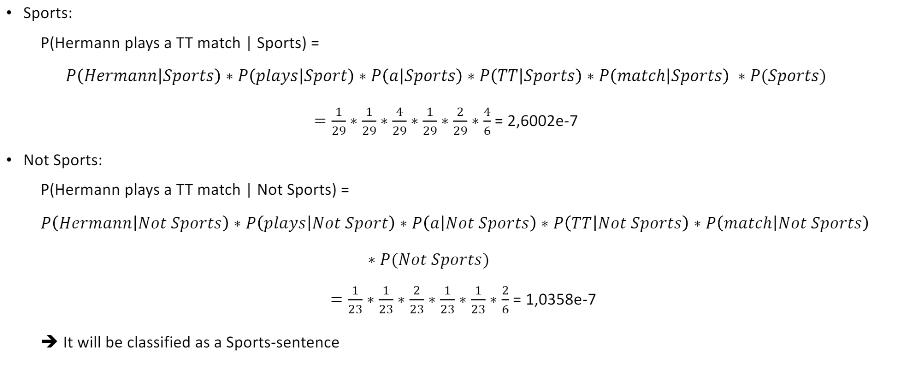
\includegraphics[width=1.1\textwidth]{Naive-Bayes-Ueb61_Hinweis}
\end{center}
\textbf{Zusatzfrage:} Das Ergebnis dreht sich rum wenn Sie als Zielsatz \textbf{"Hermann plays a very clean game"} eingeben.\\

\subsubsection{Lösungshinweise zu Übung 5.2}
....\\

Die letzten Python Codeblöcke sehen Sie im folg Screenshot: 

\begin{center} 
\hspace*{-2.2cm}
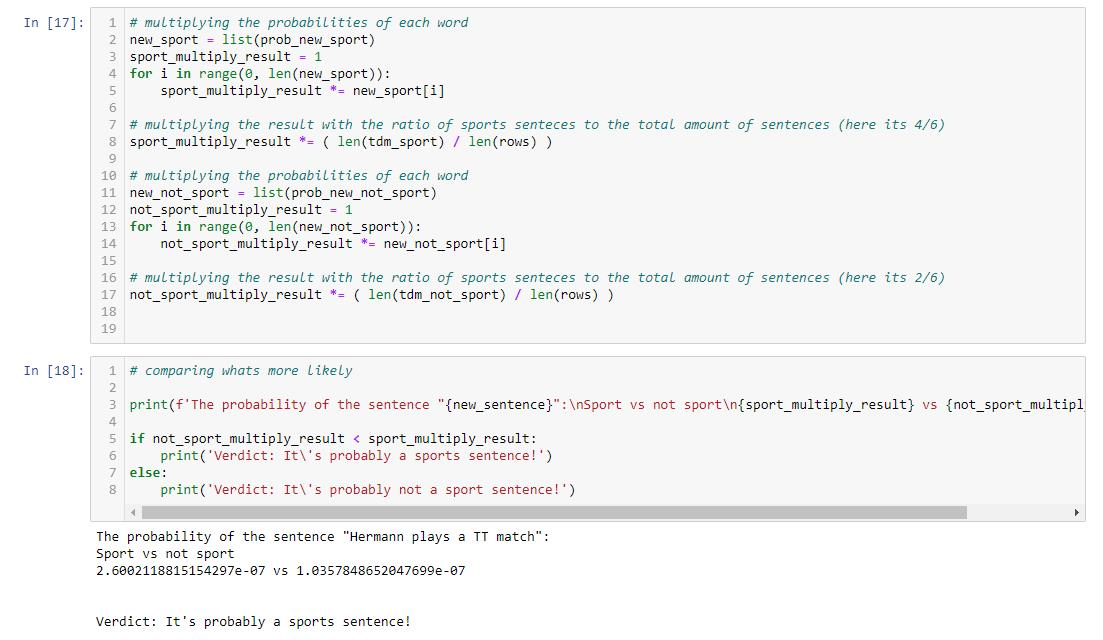
\includegraphics[width=1.3\textwidth]{Naive-Bayes-Ueb62_Hinweis}
\end{center}

\hspace*{-1.8cm} Weitere Hilfe unter \textbf{[HVö-5]} \url{https://github.com/HVoellinger/Lecture-Notes-to-ML-WS2020}\\


\subsection{Lösungshinweise zu Übungen Kapitel 6}

\subsubsection{Lösungshinweise zu Übung 6.1}

................

\subsubsection{Lösungshinweise zu Übung 6.2}


\subsubsection{Lösungshinweise zu Übung 6.3}

\begin{figure}[htp]
  \centering
  \hspace*{-0.5cm} 
  \includegraphics[width=0.9\textwidth]{Kernel-Hyperebene-Code-Bild1}
  \caption{Codeblock(1+2) zum Kernel-Trick Beispiel}
  \label{fig:SVM_Ebenen}
\end{figure}

\begin{figure}[htp]
  \centering
  \hspace*{-0.5cm} 
  \includegraphics[width=0.9\textwidth]{Kernel-Hyperebene-Code-Bild2}
  \caption{Codeblock(3) zum Kernel-Trick Beispiel}
  \label{fig:SVM_Ebenen}
\end{figure}

\newpage

\subsection{Lösungshinweise zu Übungen Kapitel 7}
.....\\
\subsubsection{Lösungshinweise zu Übung 7.1}
.....\\
\subsubsection{Lösungshinweise zu Übung 7.2}

\subsection{Lösungshinweise zu Übungen Kapitel 8}

\subsubsection{Lösungshinweise zu Übung 8.1}
.....\\
\subsubsection{Lösungshinweise zu Übung 8.2}
Weitere Kapitel Texte \\
***\\
***\\
***

\newpage

\section{Referenzen}

\textbf{Liste der Referenzen:} \\

\textbf{[HVö-1]} - Hermann Völlinger: Script of the Lecture "Introduction to Data Warehousing"; DHBW Stuttgart; WS2021; \url{http://www.dhbw-stuttgart.de/~hvoellin/}\\ 

\textbf{[HVö-2]} - Hermann Völlinger and Other: Exercises and Solutions of the Lecture "Introduction to Data Warehousing"; DHBW Stuttgart; WS2021; \url{http://www.dhbw-stuttgart.de/~hvoellin/}\\

\textbf{[HVö-3]} - Hermann Völlinger and Other: Exercises and Solutions of the Lecture ”Machine Learning: Concepts and Algorithms"; DHBW Stuttgart; WS2020; \url{http://www.dhbw-stuttgart.de/~hvoellin/}\\

\textbf{[HVö-4]} - Hermann Völlinger: Script of the Lecture "Machine Learning: Concepts and Algorithms"; DHBW Stuttgart; WS2020; \url{http://www.dhbw-stuttgart.de/~hvoellin/}\\ 

\textbf{[HVö-5]} - Hermann Völlinger: GitHub to the Lecture "Machine Learning: Concepts and Algorithms"; \url{https://github.com/HVoellinger/Lecture-Notes-to-ML-WS2020}\\

\textbf{[DHBW-Moodle]} - DHBW-Moodle for TINF19D: "Directory of supporting Information for the DWH Lecture"; \textit{Kurs: T3INF4304-3-Data Warehouse (dhbw-stuttgart.de)}\\

\textbf{[Hands-on ML]} - Aurelien Geron "Hands-on Machine Learning with SciKit-Learn, Keras and Tensorflow"; Paperback, O'Reilly (2nd edition), 2019\\

\textbf{[DL for NLP]} - Kamath, Liu and Whitaker "Deep Learning for NLP and Speech Recognition"; Paperback, Springer Verlag, 2019.\\

\textbf{[LA and Opt for ML]} - Charu C. Aggarwal "Linear Algebra and Optimization for Machine Learning"; Paperback, Springer Verlag, 2020.\\

\textbf{[Math for DL]} - Berner, Grohs, Kutyniok, and Petersen: "The Modern Mathematics of Deep Learning"; Review Paper; ResearchGate arXiv:2105.04026v1 [cs.LG] 9 May 2021; This review paper will appear as a book chapter in the book "Theory of Deep Learning" by Cambridge University Press\\

\textbf{[SVM-Def]} - "Was ist eine Support Vector Machine?"; 06.11.2019; Autor, Redakteur: Dipl.-Ing. (FH) Stefan Luber / Nico Litzel; \url{https://www.bigdata-insider.de/was-ist-eine-support-vector-machine-a-880134/}\\

\textbf{[TK + SVM]} - Seminararbeit von Alena Tabea Geduldig: "Textklassifikation mit Support Vector Machines" im  Hauptseminar "Linguistic Software Engineering“ bei Prof. Dr. Jürgen Rolshoven (Uni Köln); WS 2014/2015; \url{https://docplayer.org/9656155-Textklassifikation-mit-support-vector-machines.html}\\

\textbf{[BackP-Exam]} - "A Step by Step Backpropagation Example" by Matt Mazur (2018); \url{https://mattmazur.com/2015/03/17/a-step-by-step-backpropagation-example/}\\

\textbf{[BackP-Scikit]} - "Scikit-learn 0.23.1; Ch. 1.17. Neural network models (supervised)";\url{https://github.com/mattm/simple-neural-network}\\

\textbf{[Wiki-ML]} - Wikipedia: "Machine learning ML); \url{https://en.wikipedia.org/wiki/Machine_learning}{Machine Learning}\\

\textbf{[Wiki-SVM]} - Wikipedia: Support Vector Machine (SVM); \url{https://de.wikipedia.org/wiki/Support Vector Machine(SVM)} \\

*** Weitere Referenzen \\
***\\


\end{document}